\section{Oživení a obsluha}
\label{sec:ovladani}
Příprava ke spuštění probíhá v několika krocích:
\begin{enumerate}
  \item Připraví se centrální jednotka (v tomto případě switch) a k ní se pomocí síťového kabelu připojí všechna zařízení (klienti i server). Zapojení znázorněno na obrázku \ref{fig:schema_net}.

  \item Připojit napájení k serveru i klientům, pro server napájení 6~-~16~V~DC schopné dodat alespoň 250~mA, pro klienty 6~-~25~V~DC alespoň 500~mA.

  \item Pokud je vše v pořádku, na serveru svítí svítivá dioda modrou barvou a na displejích klientů je úvodní obrazovka s tlačítkem \uv{\textit{PRIPOJIT}} (viz. obrázek \label{fig:faze1}).
\end{enumerate}

\subsection{Ovládání klienta}
\begin{enumerate}
\item Po úspěšném zapnutí se vykreslí úvodní obazovka. (obrázek:~\ref{fig:faze1}).  Zobrazeny jsou informace o nastavené IP adrese serveru a o IP adrese klienta (podle režimu přiřazena DHCP serverem nebo ručně).
\begin{figure}[H]
\centering
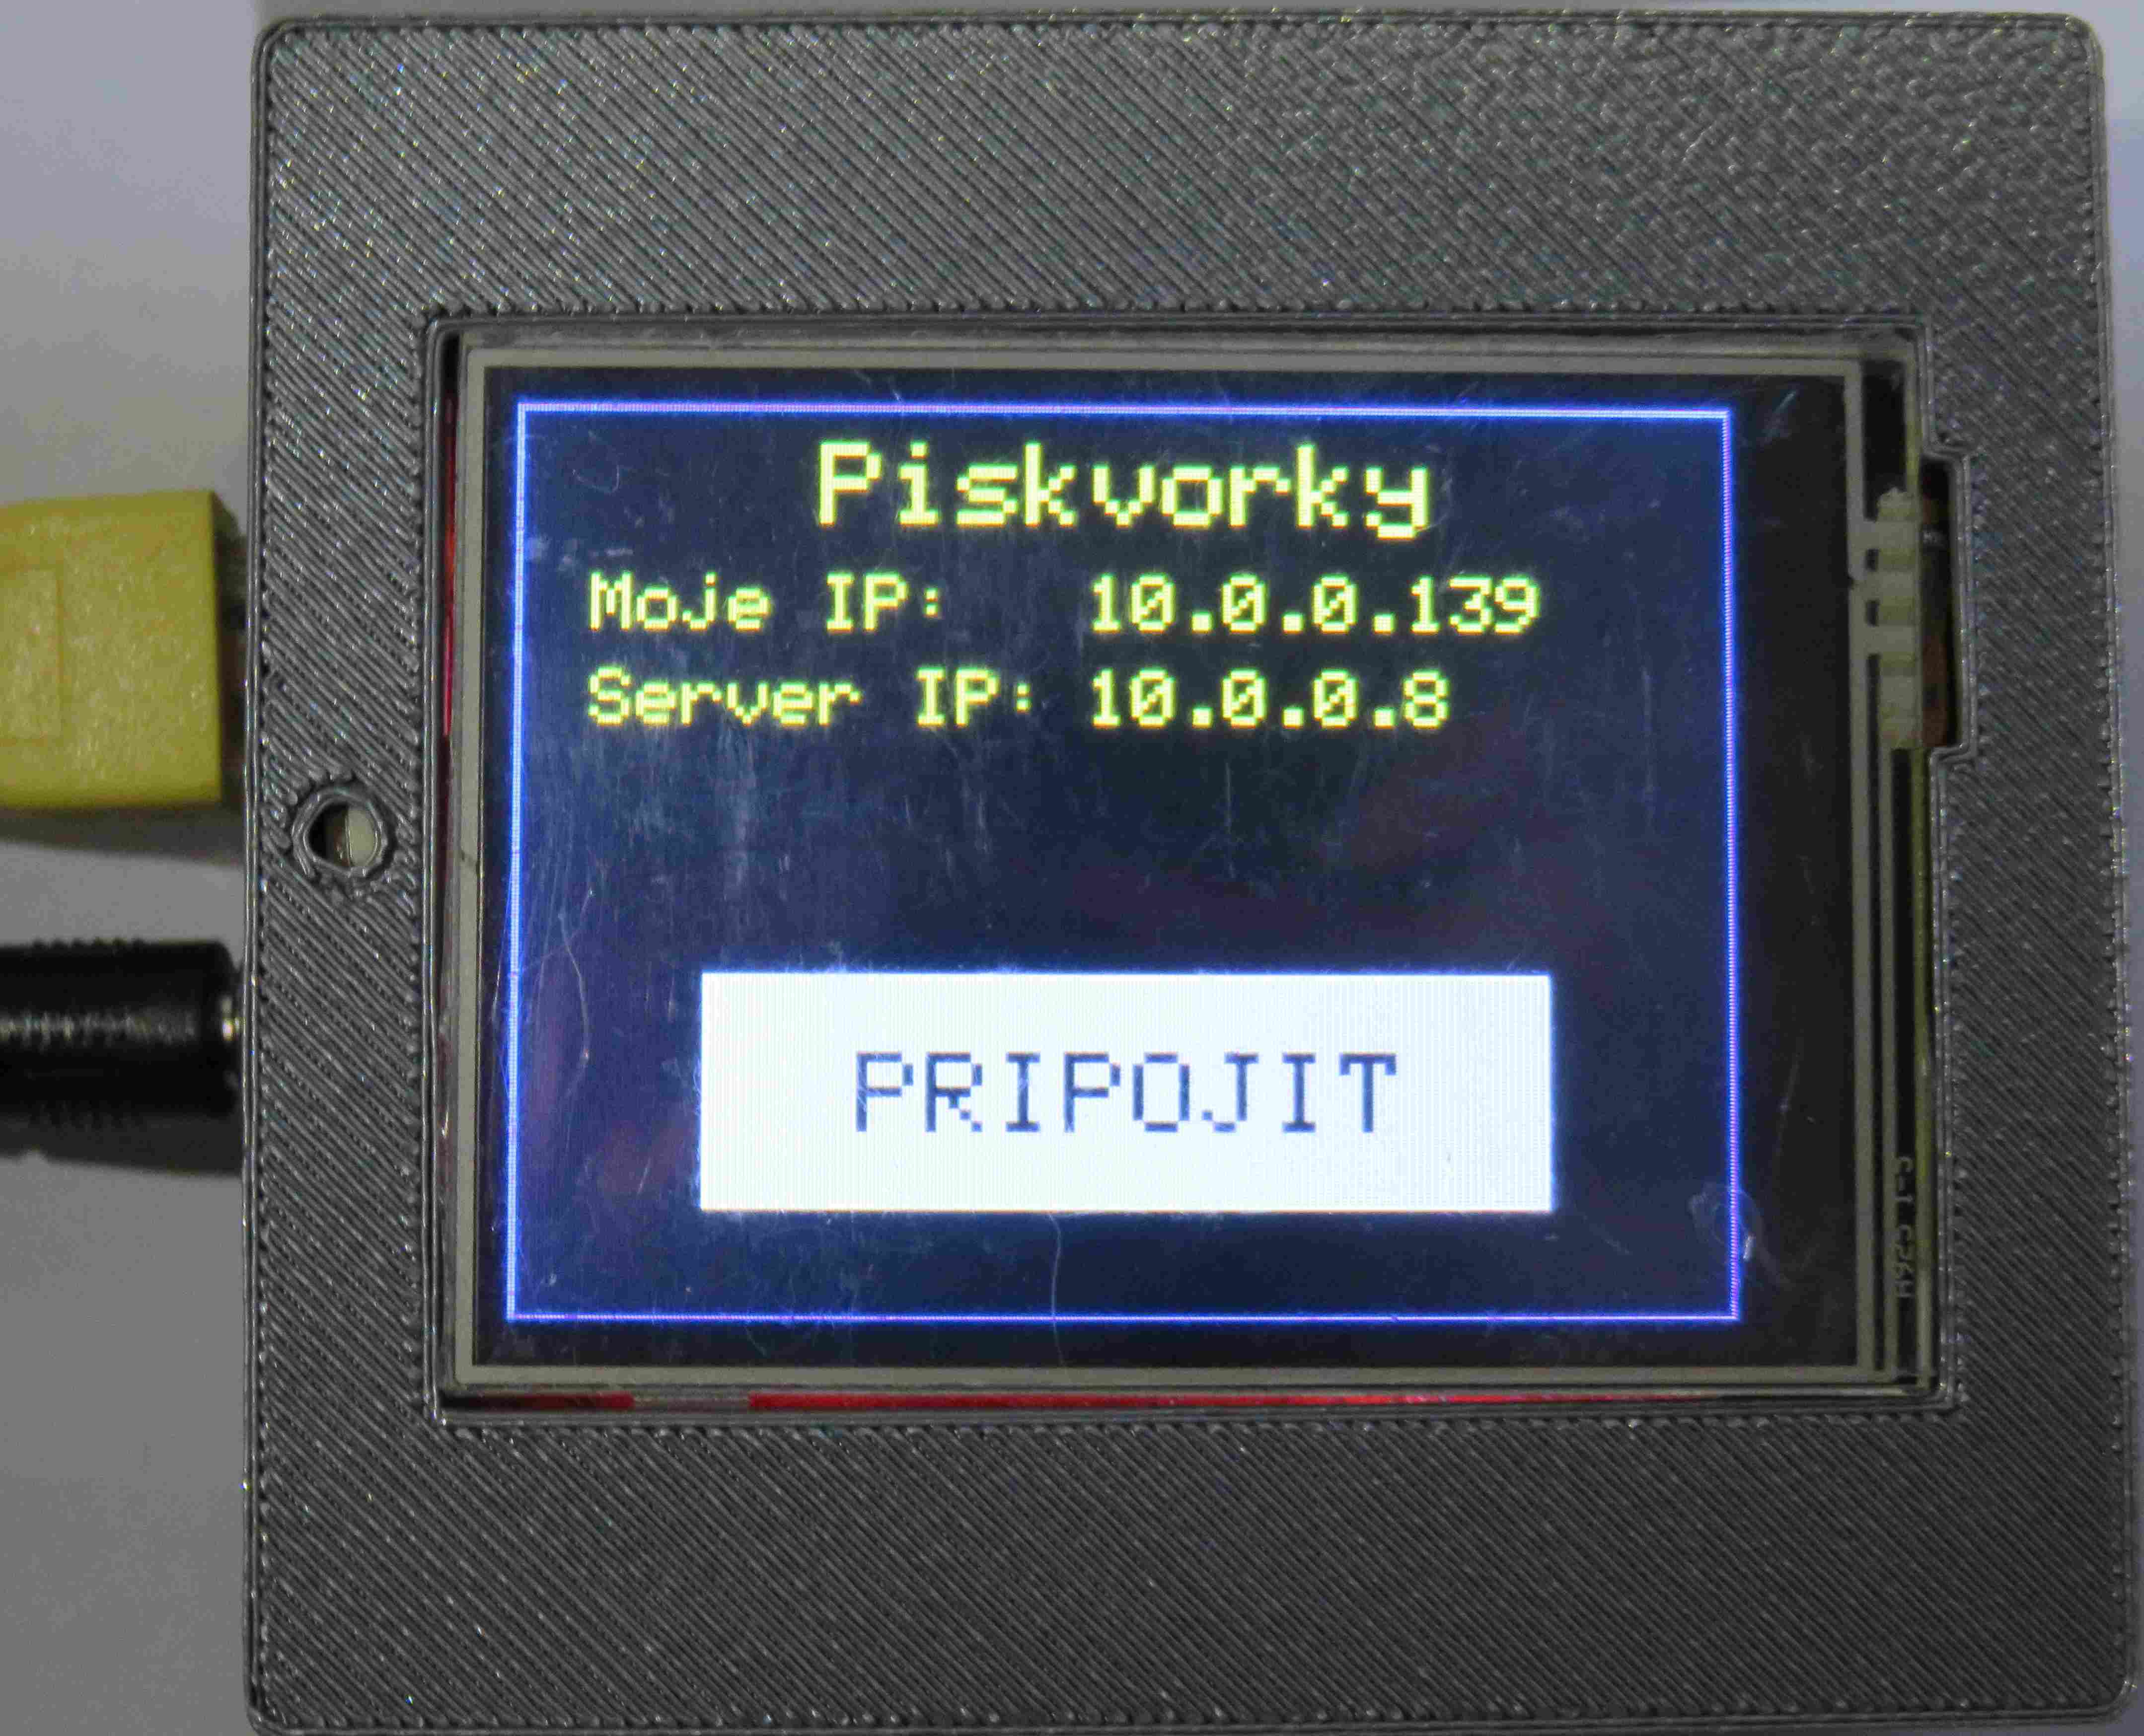
\includegraphics[width=8cm]{img/gameFlow/phase01.jpg}
\caption{\label{fig:faze1} Obrazovka klienta po úspěšném spuštění}
\end{figure}

%%%
\item Připojení k piškvorkovému serveru lze spustit stisknutím tlačítka \uv{\textit{PRIPOJIT}}. Připojování je indikováno pomocí displeje (obrázek~\ref{fig:faze2}). Připojování může být kdykoliv přerušeno stiskem tlačítka \uv{\textit{PRERUSIT}}. Připojování bude dokončeno pokud na serveru není rozehraná hra.
\begin{figure}[H]
\centering
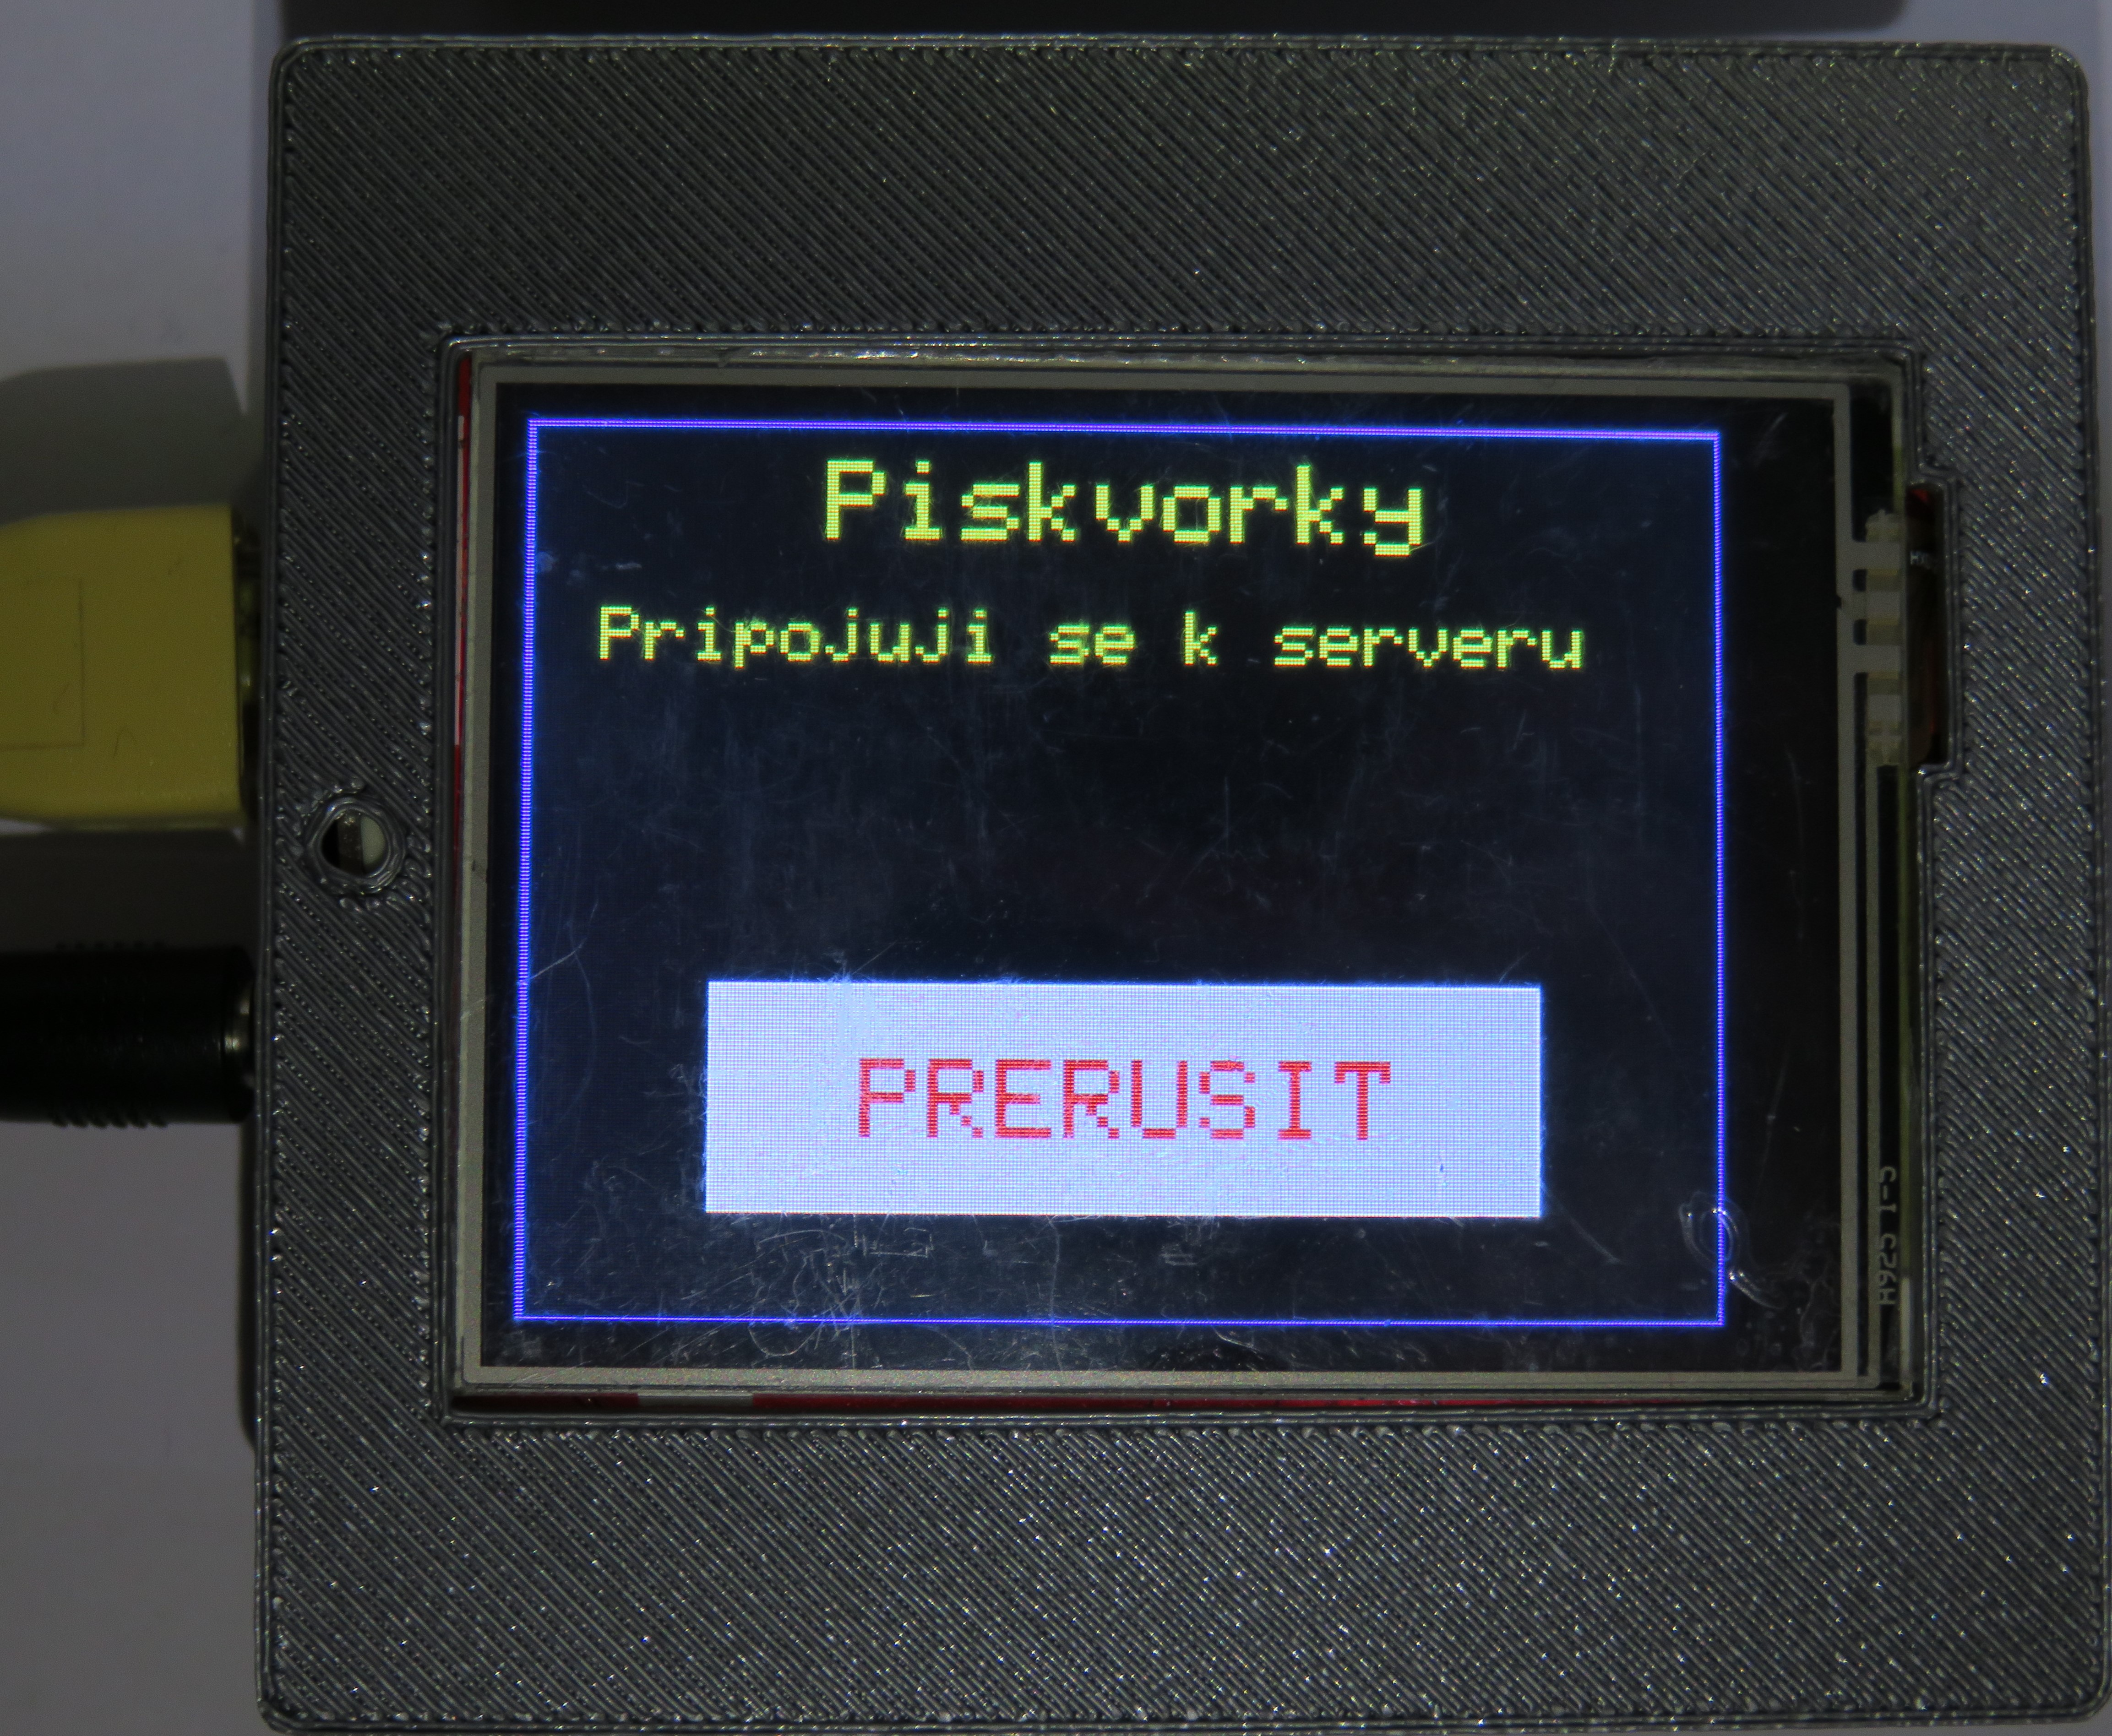
\includegraphics[width=8cm]{img/gameFlow/phase02.jpg}
\caption{\label{fig:faze2} Obrazovka klienta při připojování k serveru}
\end{figure}

%%%
\item Pokud připojení proběhlo úspěšně, klient má od serveru přiřazené číslo a barvu. To je indikováno pomocí displeje (obrázek~\ref{fig:faze3}), kde barva textu odpovídá barvě hráče. Než započne hra je možné se ze serveru odpojit stiskem tlačítka \uv{\textit{ODPOJIT}}. Nyní se čeká na zahájení hry.
\begin{figure}[H]
\centering
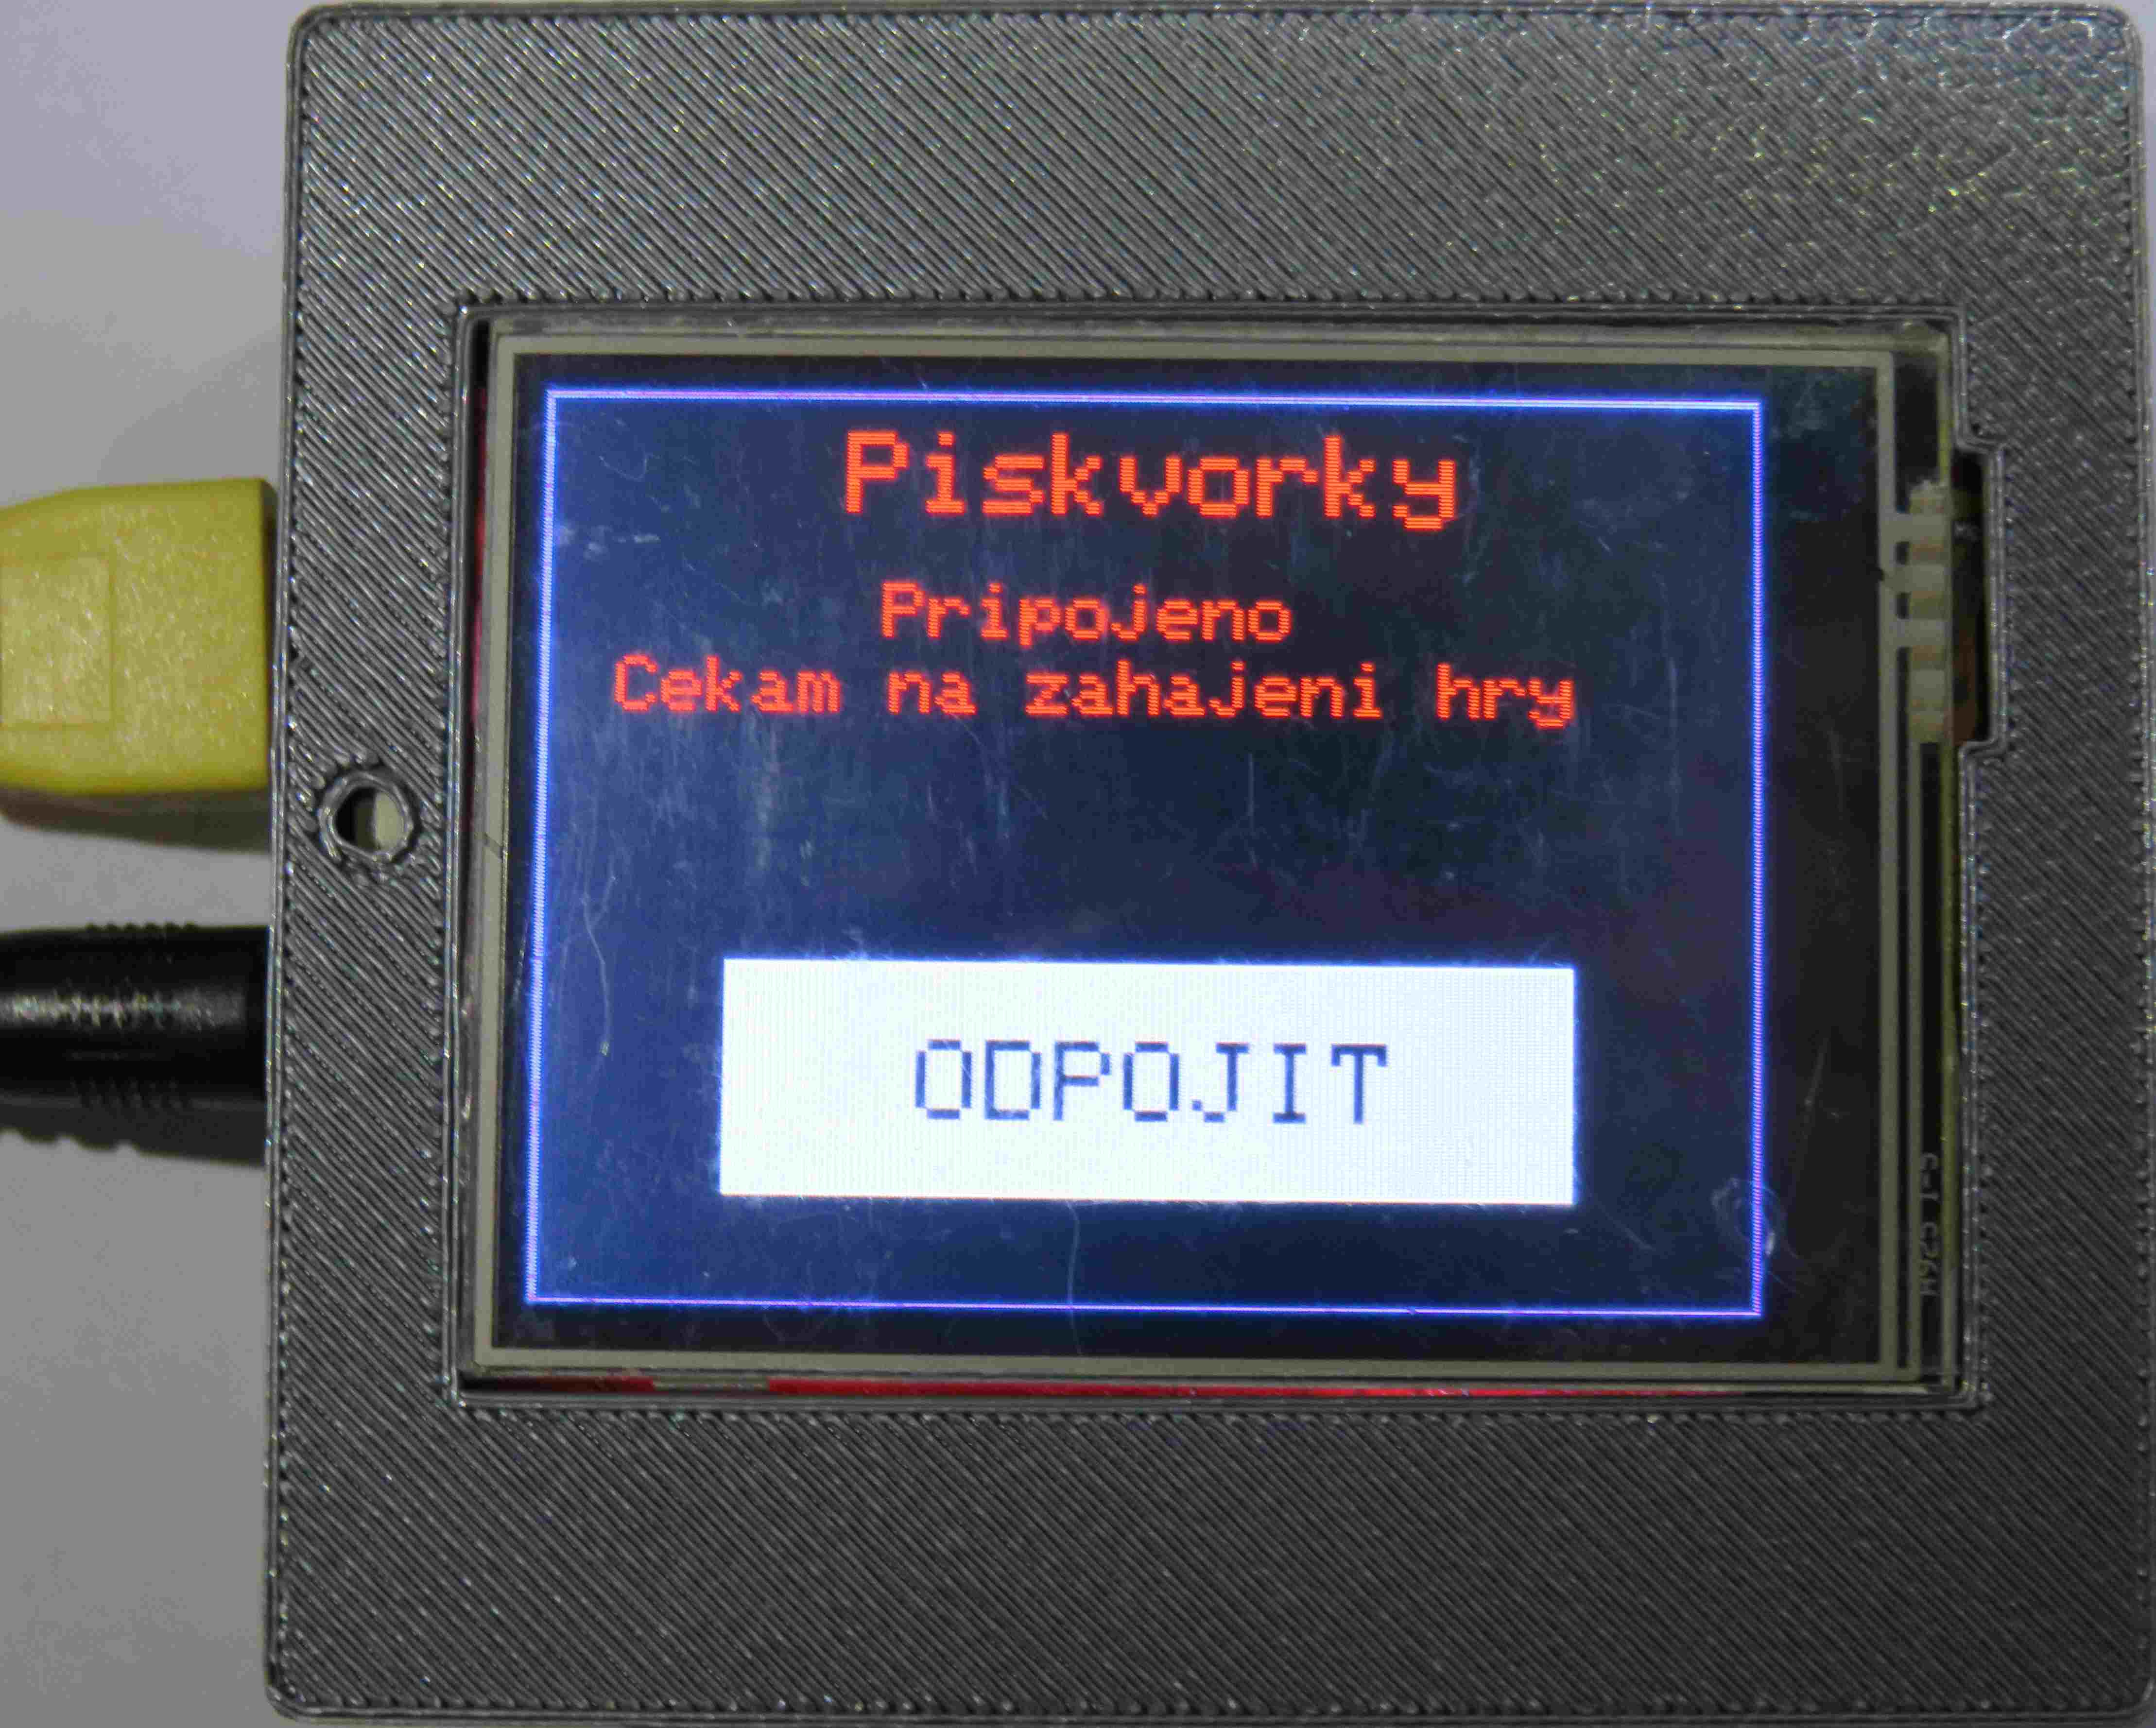
\includegraphics[width=7cm, angle=0]{img/gameFlow/phase03a.jpg}
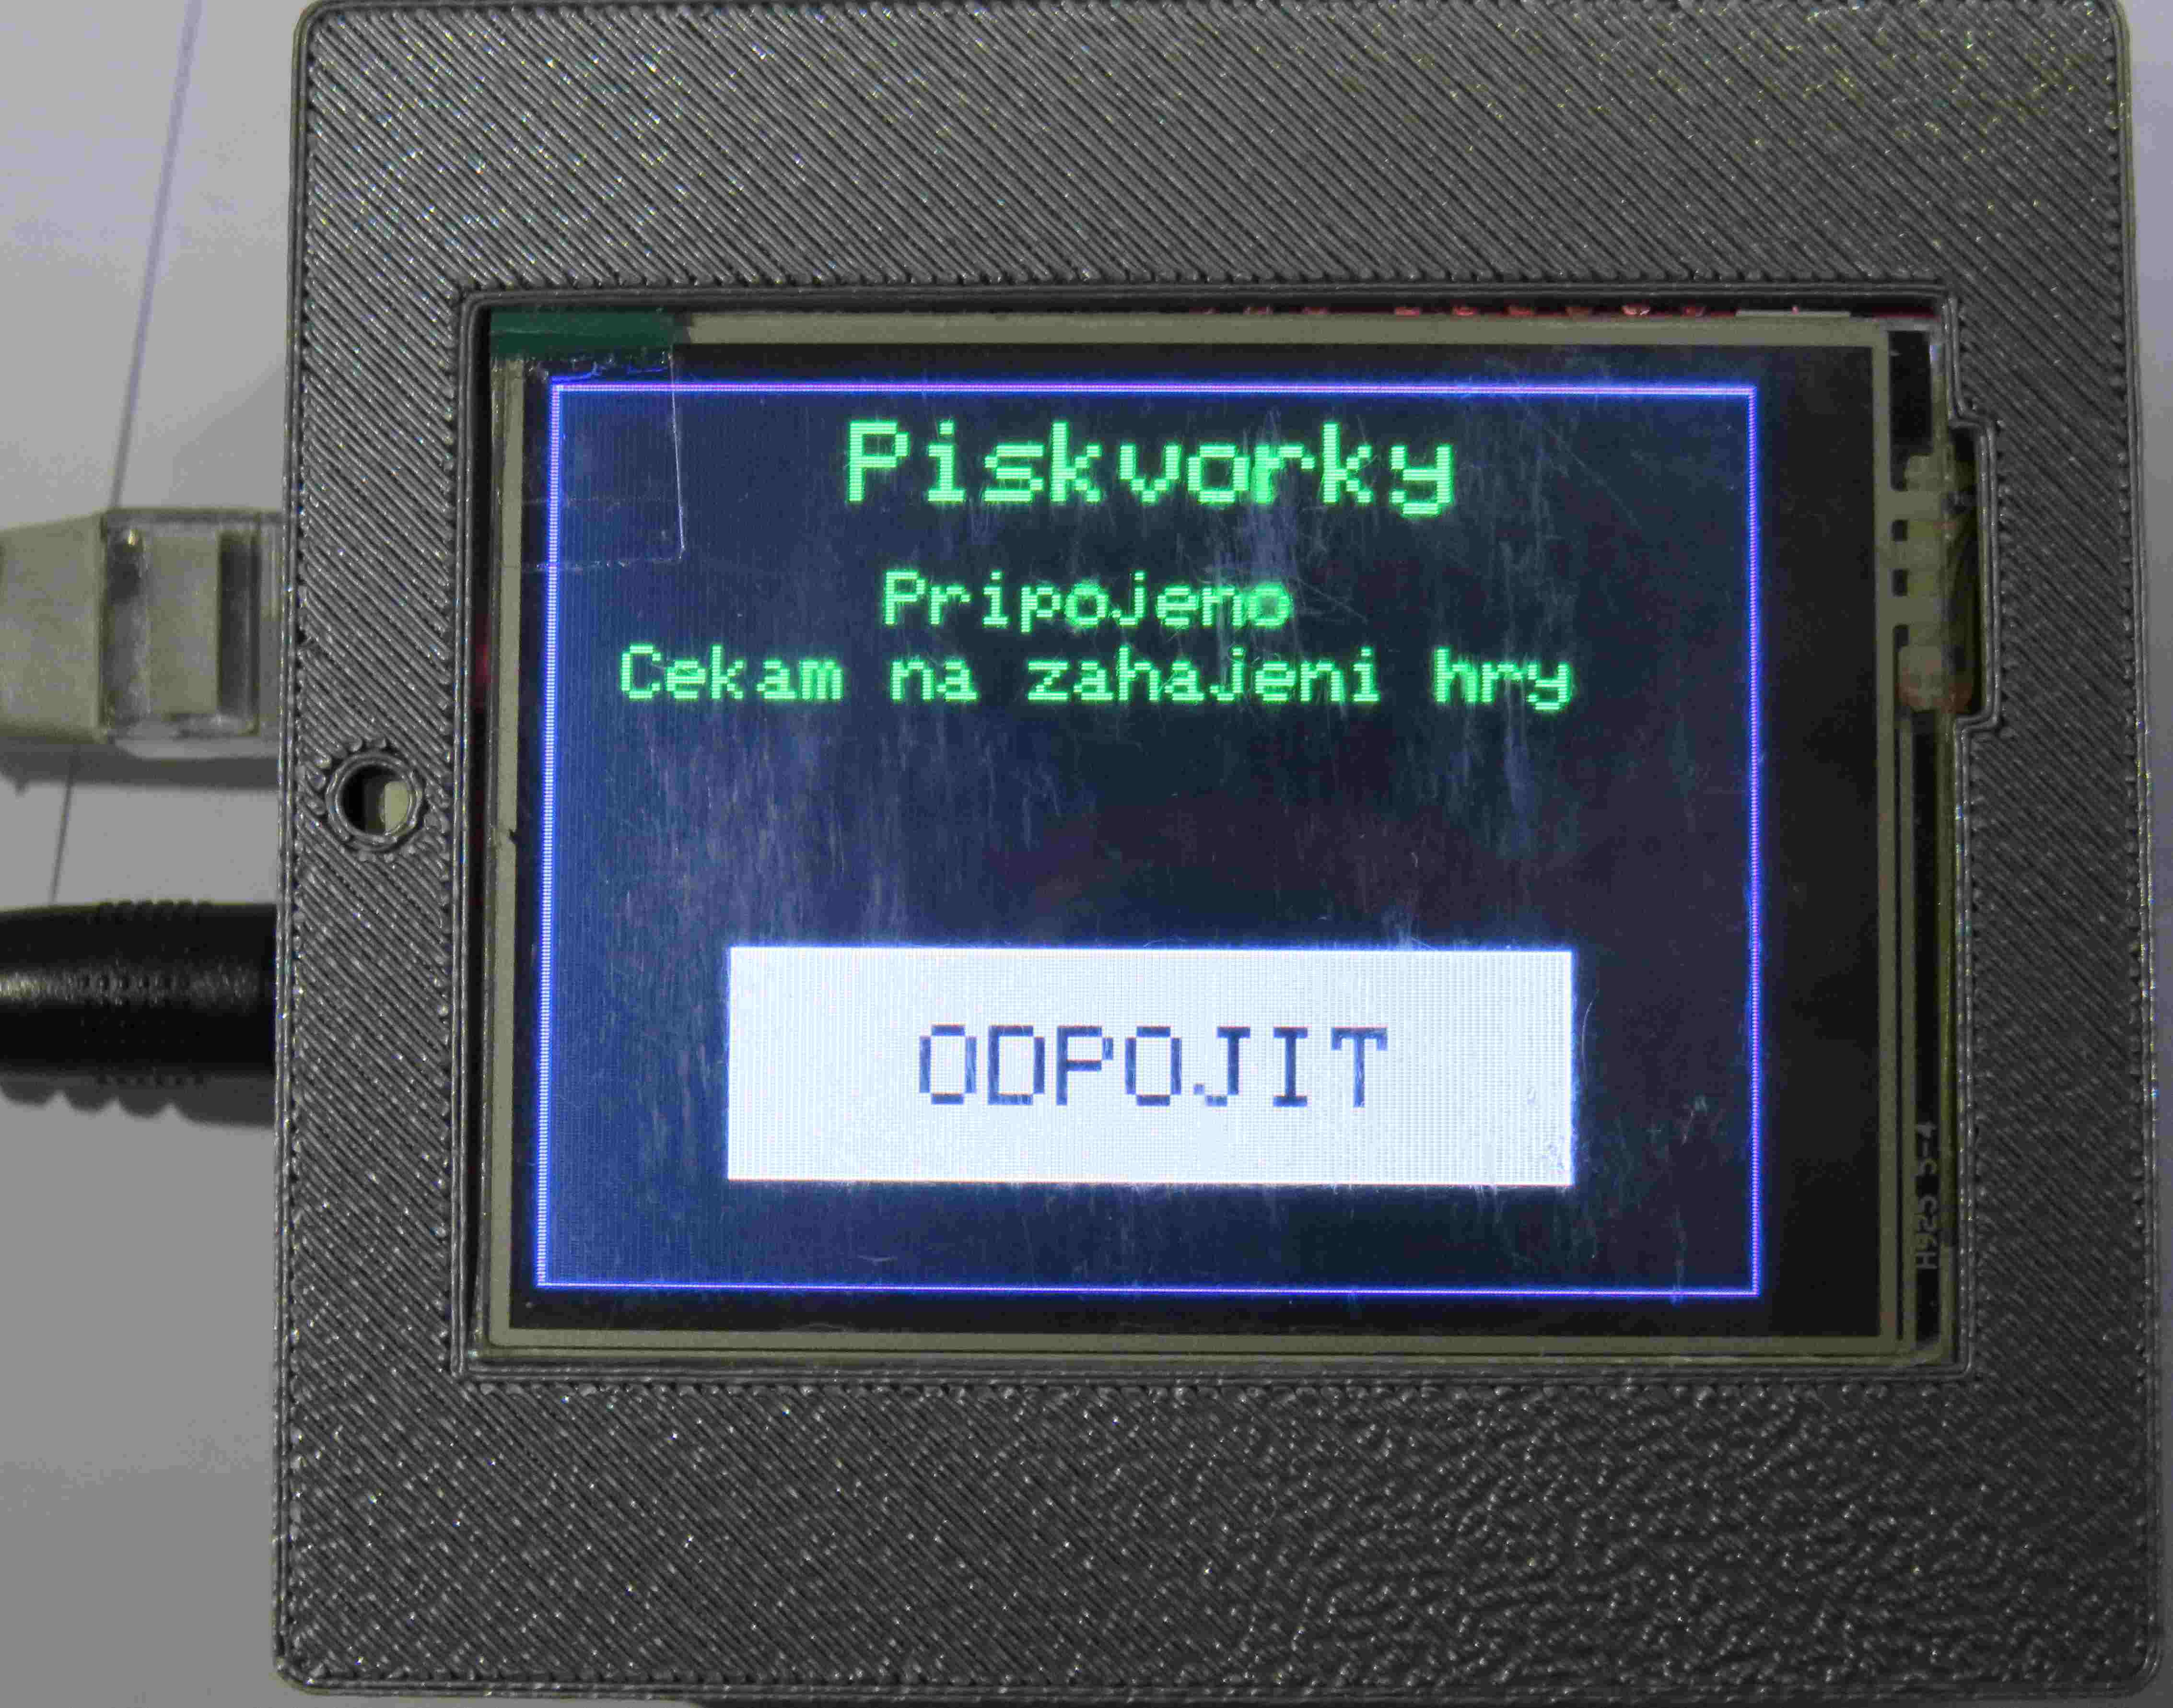
\includegraphics[width=7cm, angle=0]{img/gameFlow/phase03b.jpg}
\caption{\label{fig:faze3} Obrazovky dvou různých klientů  po úspěšném připojení k piškvorkovému serveru}
\end{figure}
\label{item:faze3}

%%%
\item V případě, že ze strany serveru byla započata hra (příkazem nebo stiskem zeleného tlačítka), vykreslí se na obrazovce herní pole (obrázek~\ref{fig:faze4}).

Jednotlivé čtverce mají pro tento typ displeje fyzický rozměr přibližně 0,5x0,5~mm. Tato velikost byla zvolena proto, že je možné na takto malý displej umístit dostatečně velké pole (11x8 čtverců) a zárověň je možné jej bez problém ovládat stylusem a případně i prstem.
\begin{figure}[H]
\centering
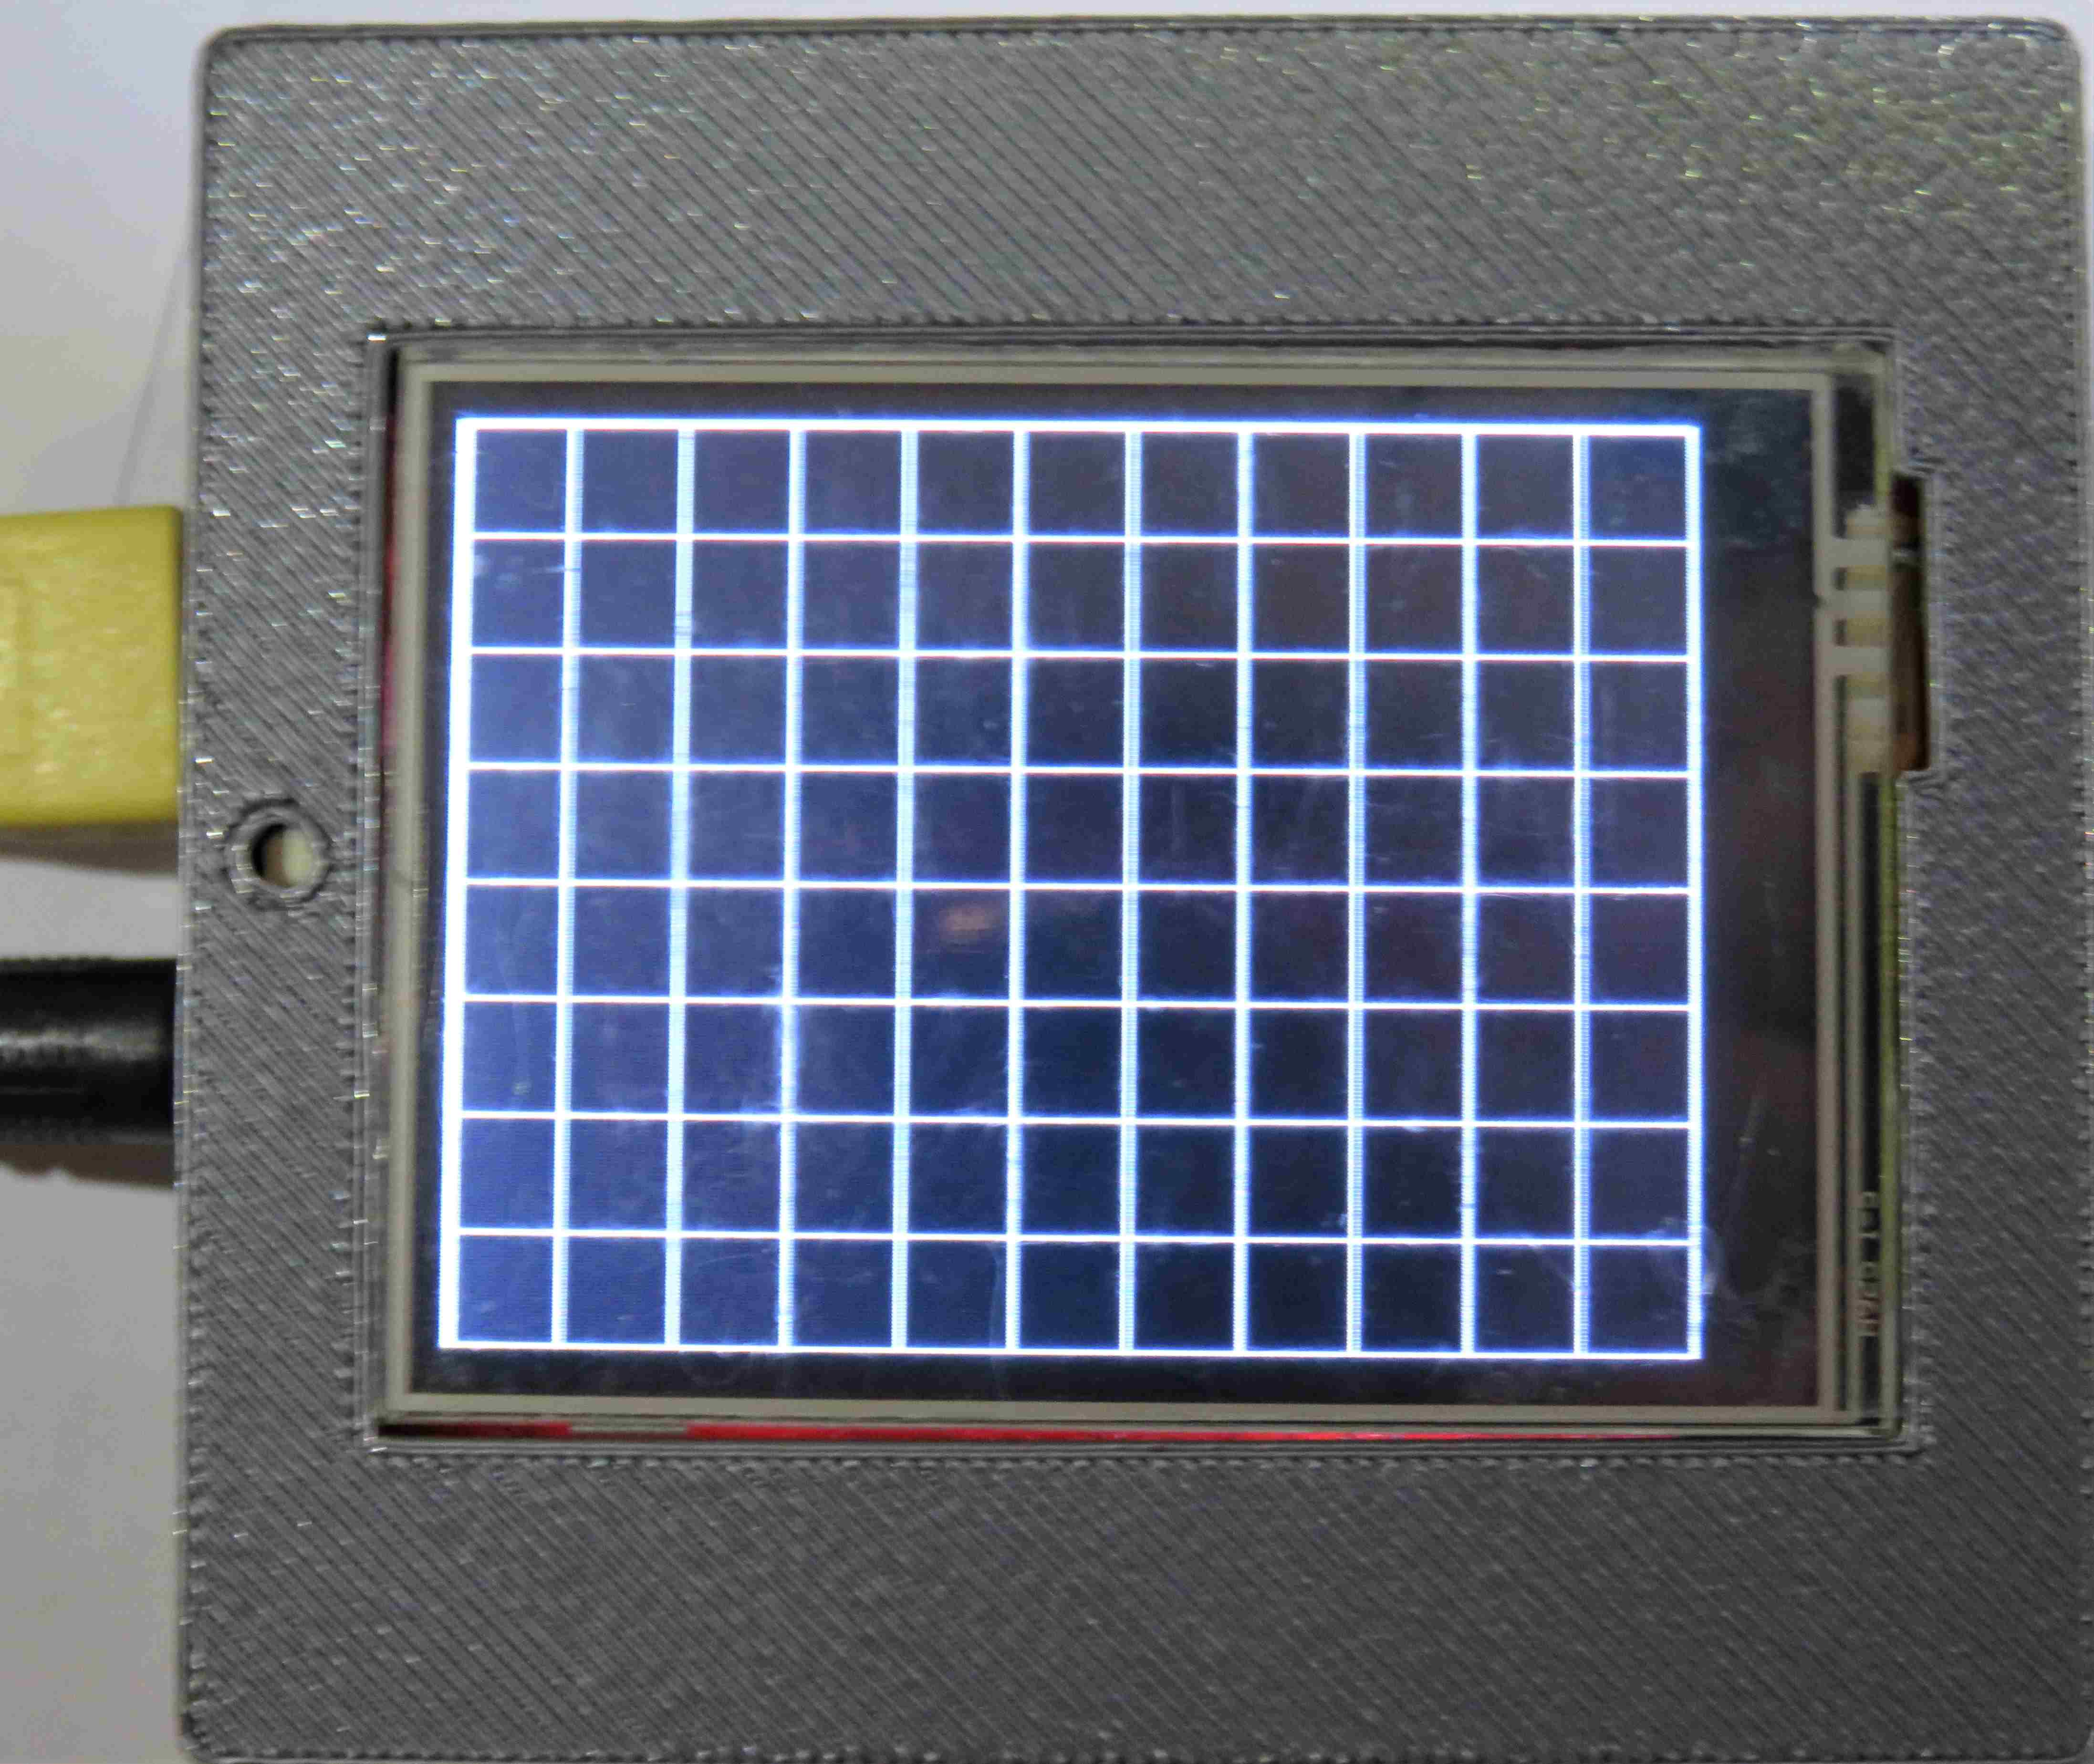
\includegraphics[width=7cm, angle=0]{img/gameFlow/phase04a.jpg}
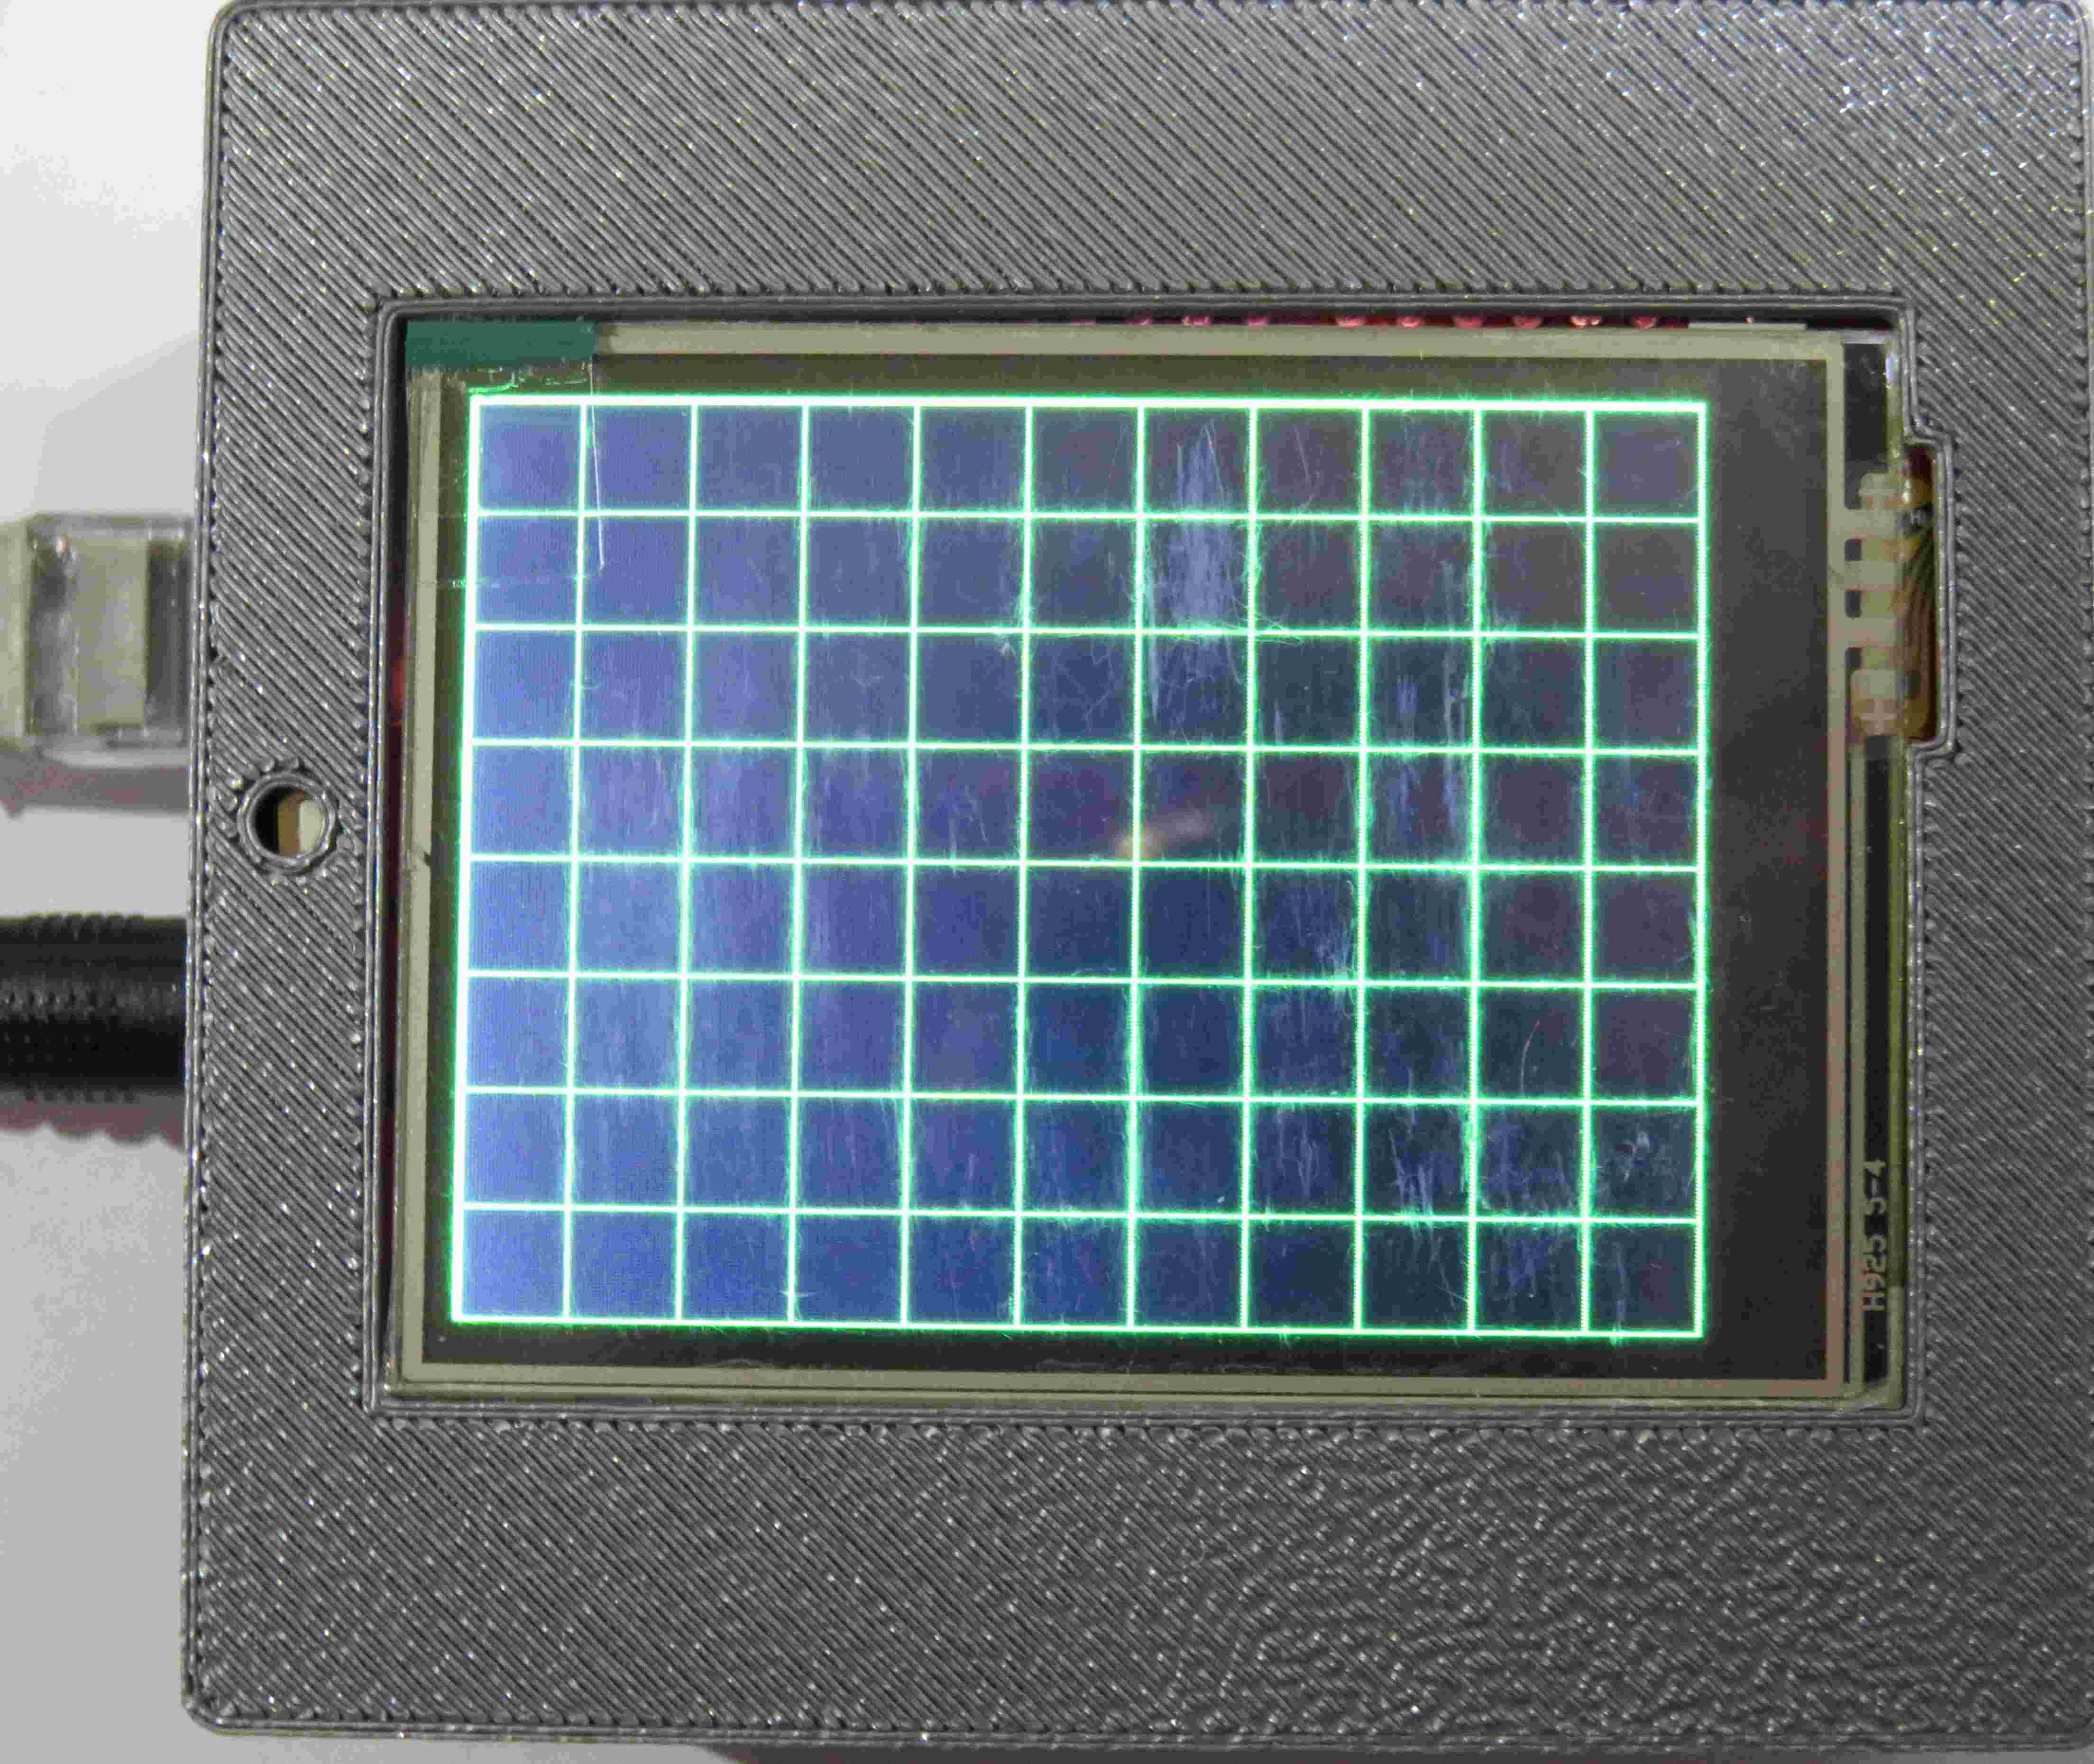
\includegraphics[width=7cm, angle=0]{img/gameFlow/phase04b.jpg}
\caption{\label{fig:faze4} Obrazovka klienta po započaté hře (a) čekající hráč, (b) hrající hráč}
\end{figure}

%%
\item Během hry: pokud je mřížky šedá, hraje jiný hráč, pokud má mřížka nějakou barvu (barva se shoduje s barvou hráče) je na tahu daný hráč. Ten má za úkol stiskem libovolného volného čtverečku umístit svůj žeton.

Když uživatel stiskne čtverec, dojde k jeho vyplnění příslušným žetonem (barevným kruhem), mříž zešedne a je na řadě další hráč. Rozehraná hra je vidět na obrázku~\ref{fig:faze5}.
\begin{figure}[H]
\centering
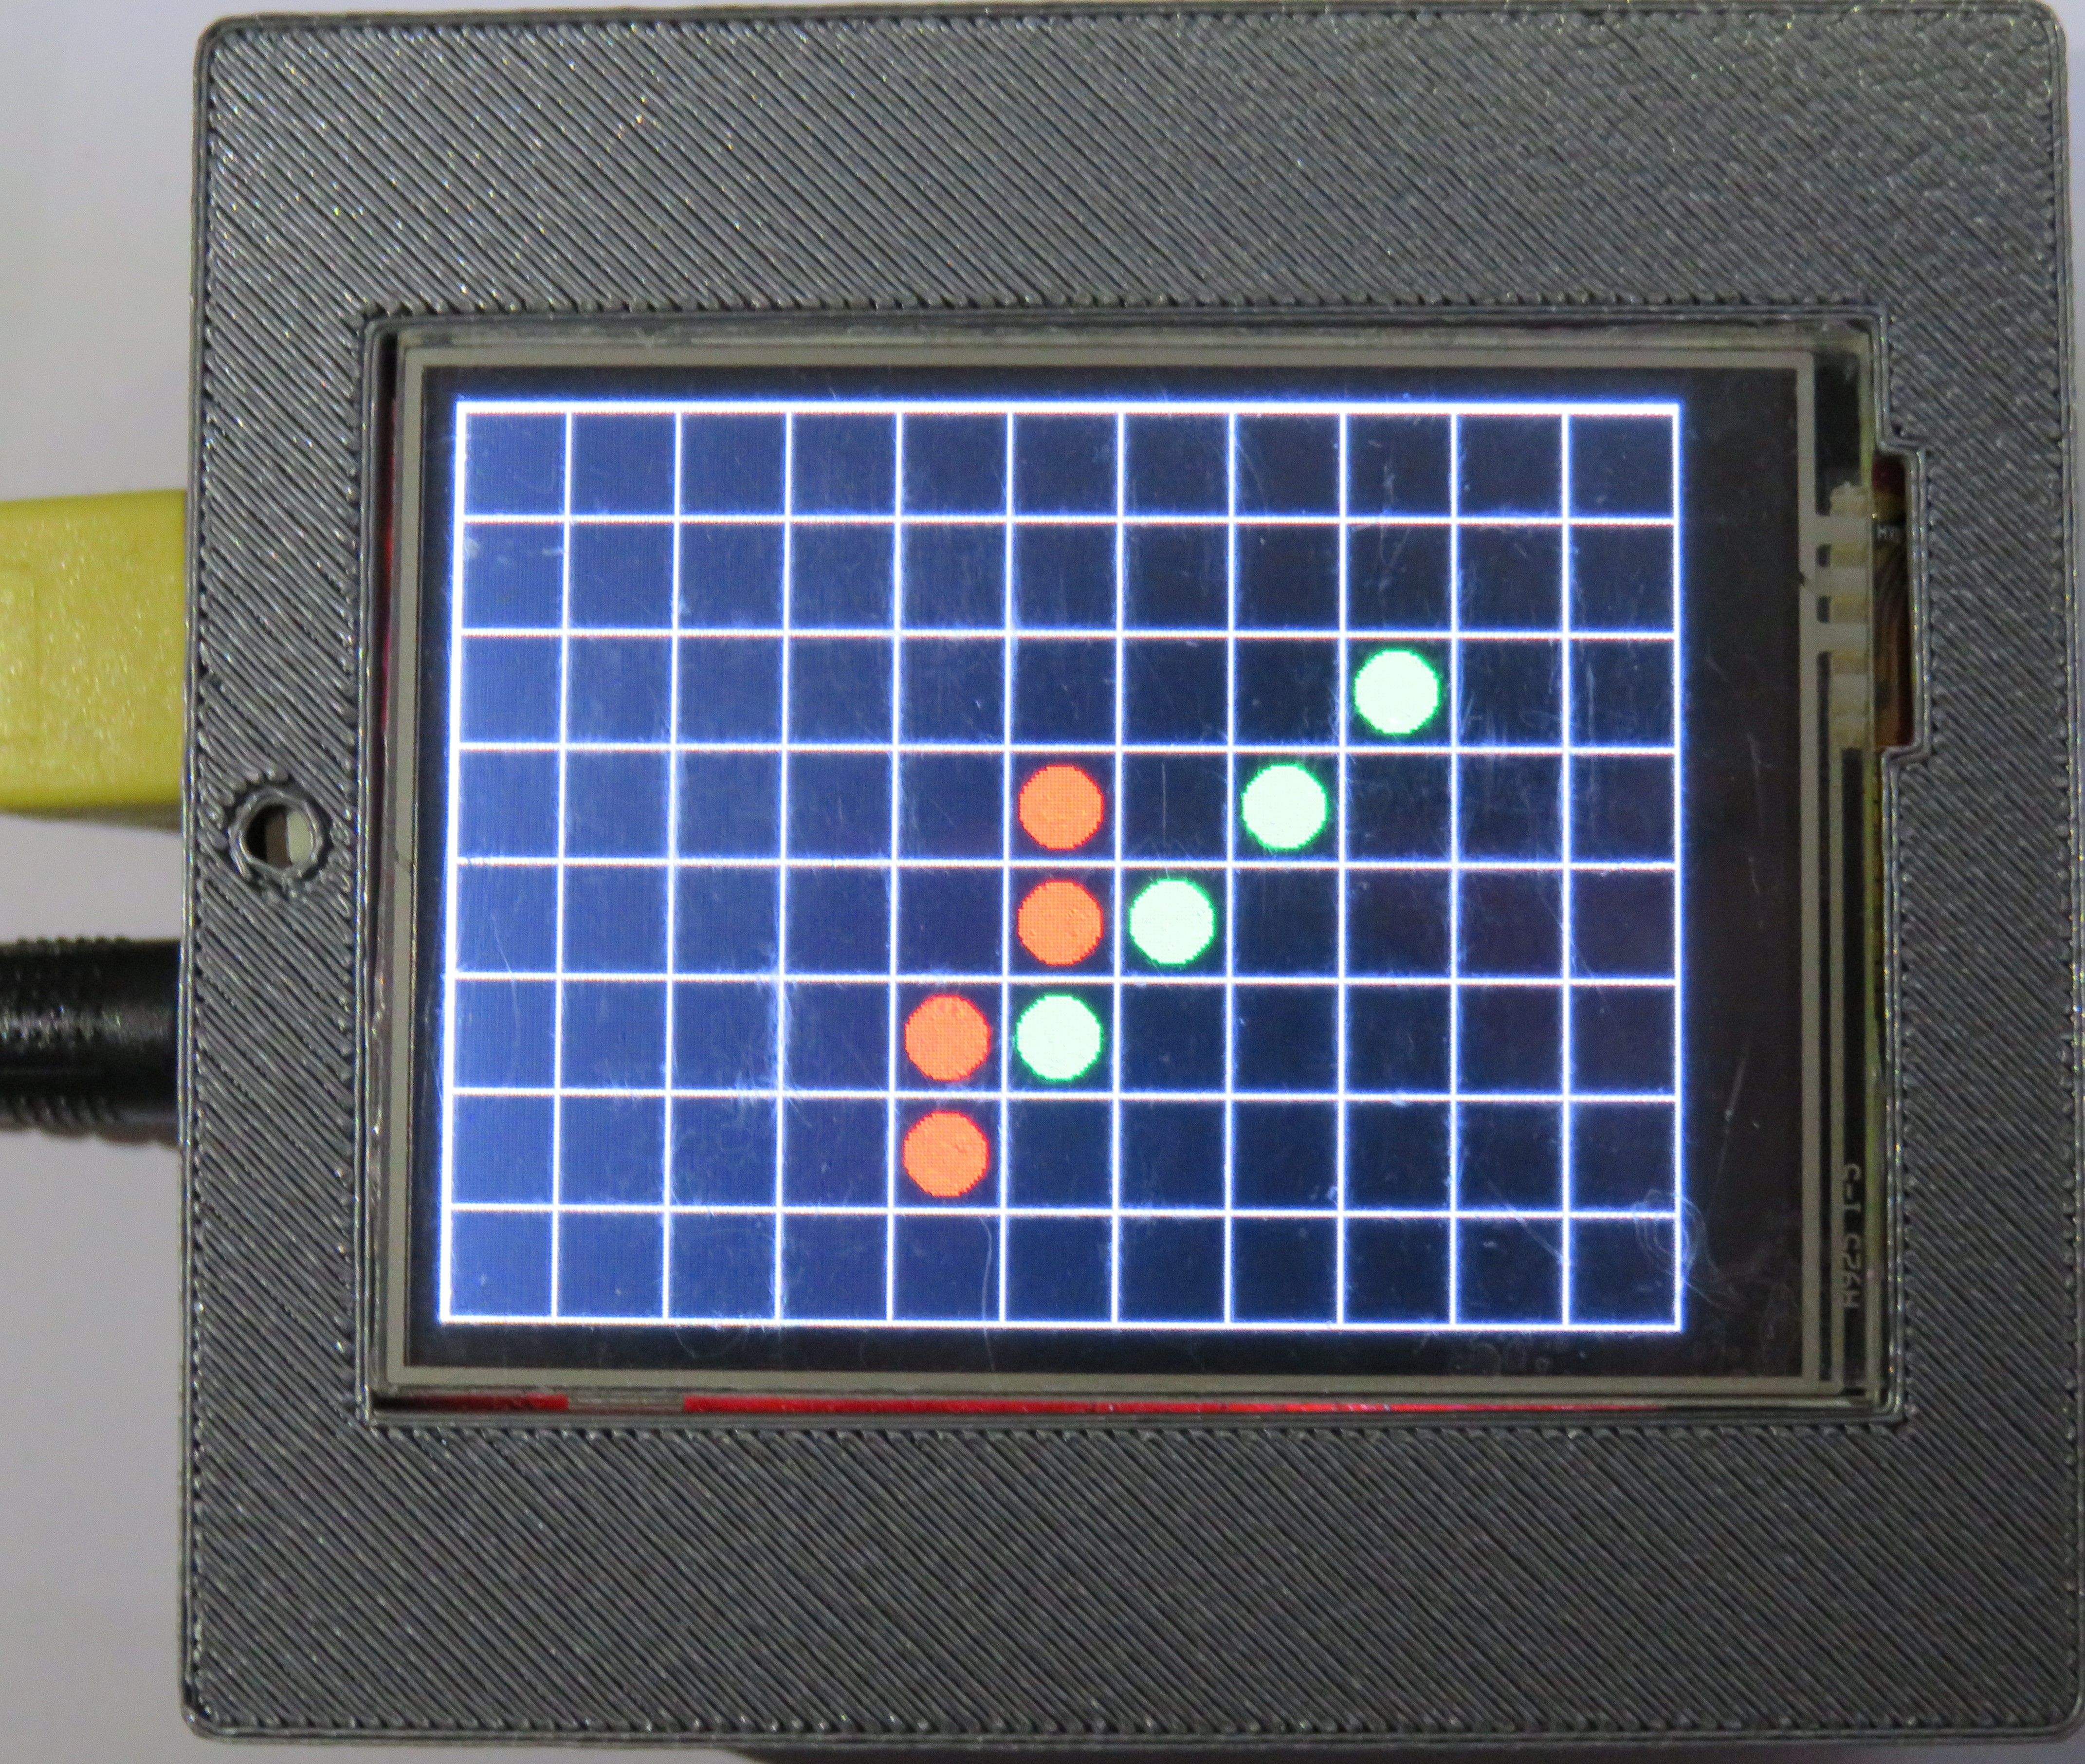
\includegraphics[width=7cm, angle=0]{img/gameFlow/phase05a.jpg}
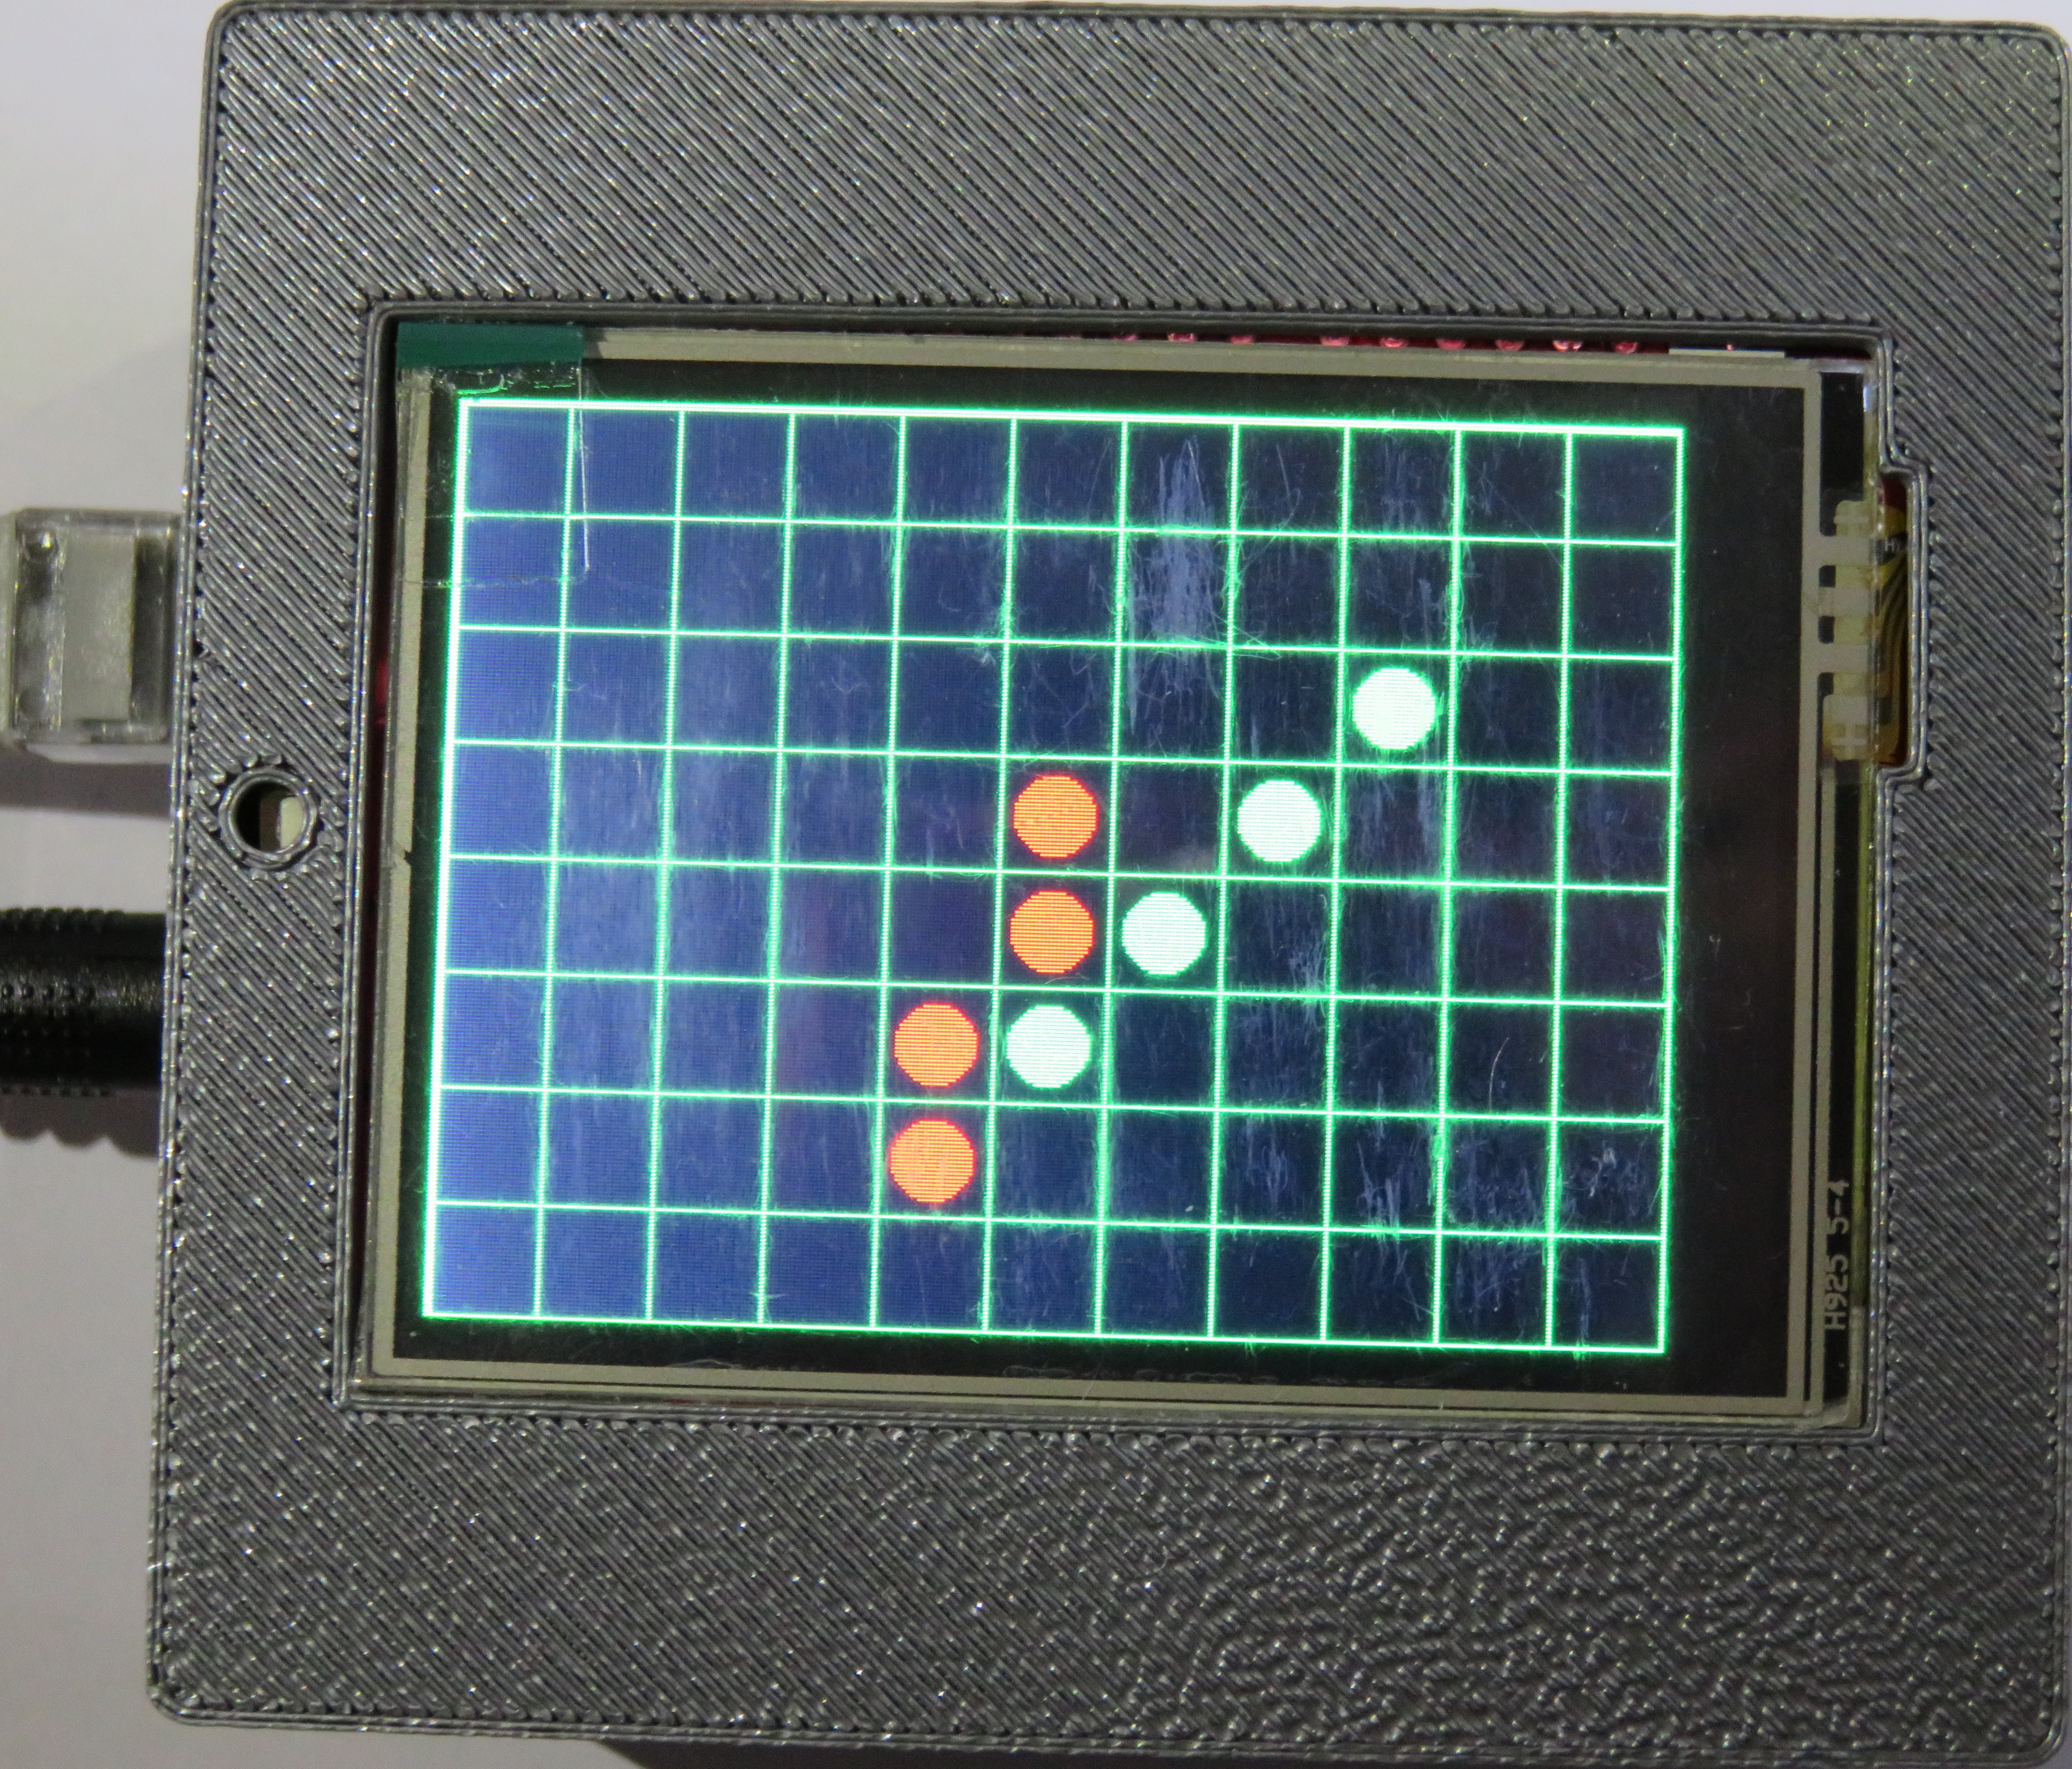
\includegraphics[width=7cm, angle=0]{img/gameFlow/phase05b.jpg}
\caption{\label{fig:faze5} Rozehraná hra dvou hráčů}
\end{figure}

%%
\item Hráči se střídají do té doby než: jsou všechna pole vyplněna (ukončeno remízou) nebo některý hráč spojil požadovaný počet žetonů (v základní nastavení pět). O výsledku hry jsou hráči informováni hláškou na displeji (obrázek~\ref{fig:faze6}). Tato hláška po deseti sekundách zmizí (nastaveno v proměnné \texttt{clientMessageLast} v milisekundách) a hra přechází do fáze~3.
\begin{figure}[H]
\centering
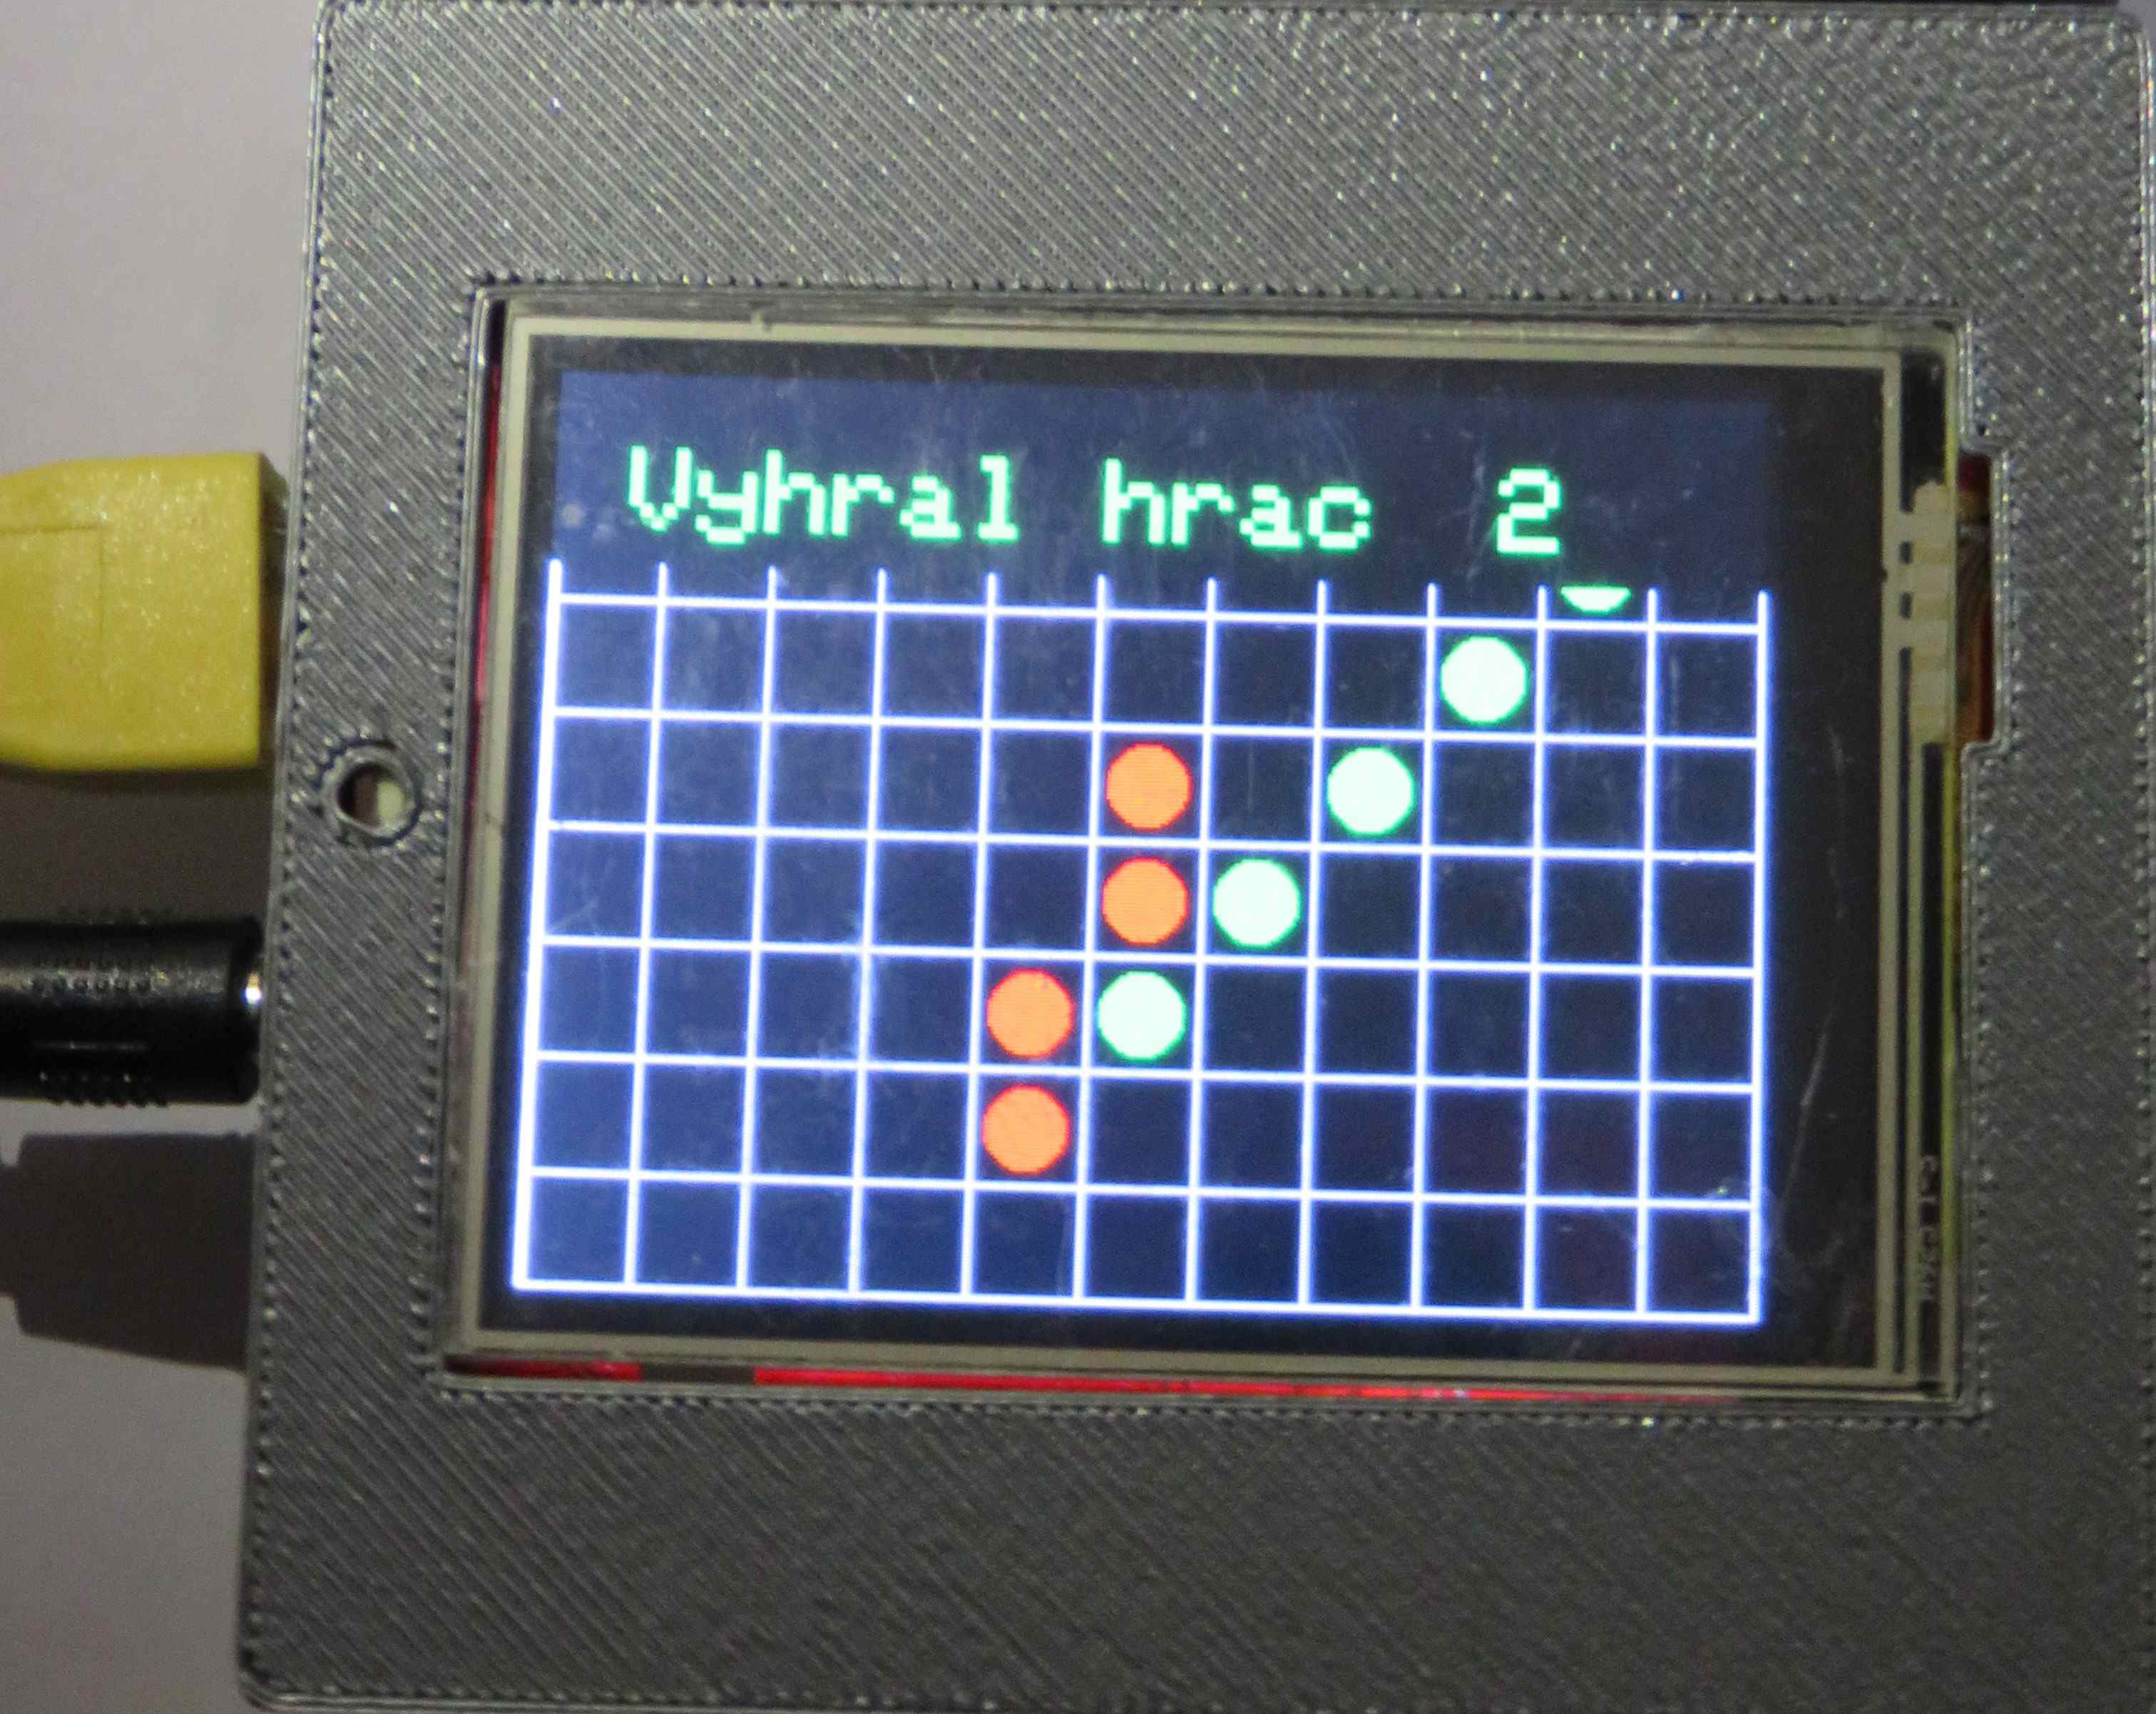
\includegraphics[width=7cm, angle=0]{img/gameFlow/phase06a.jpg}
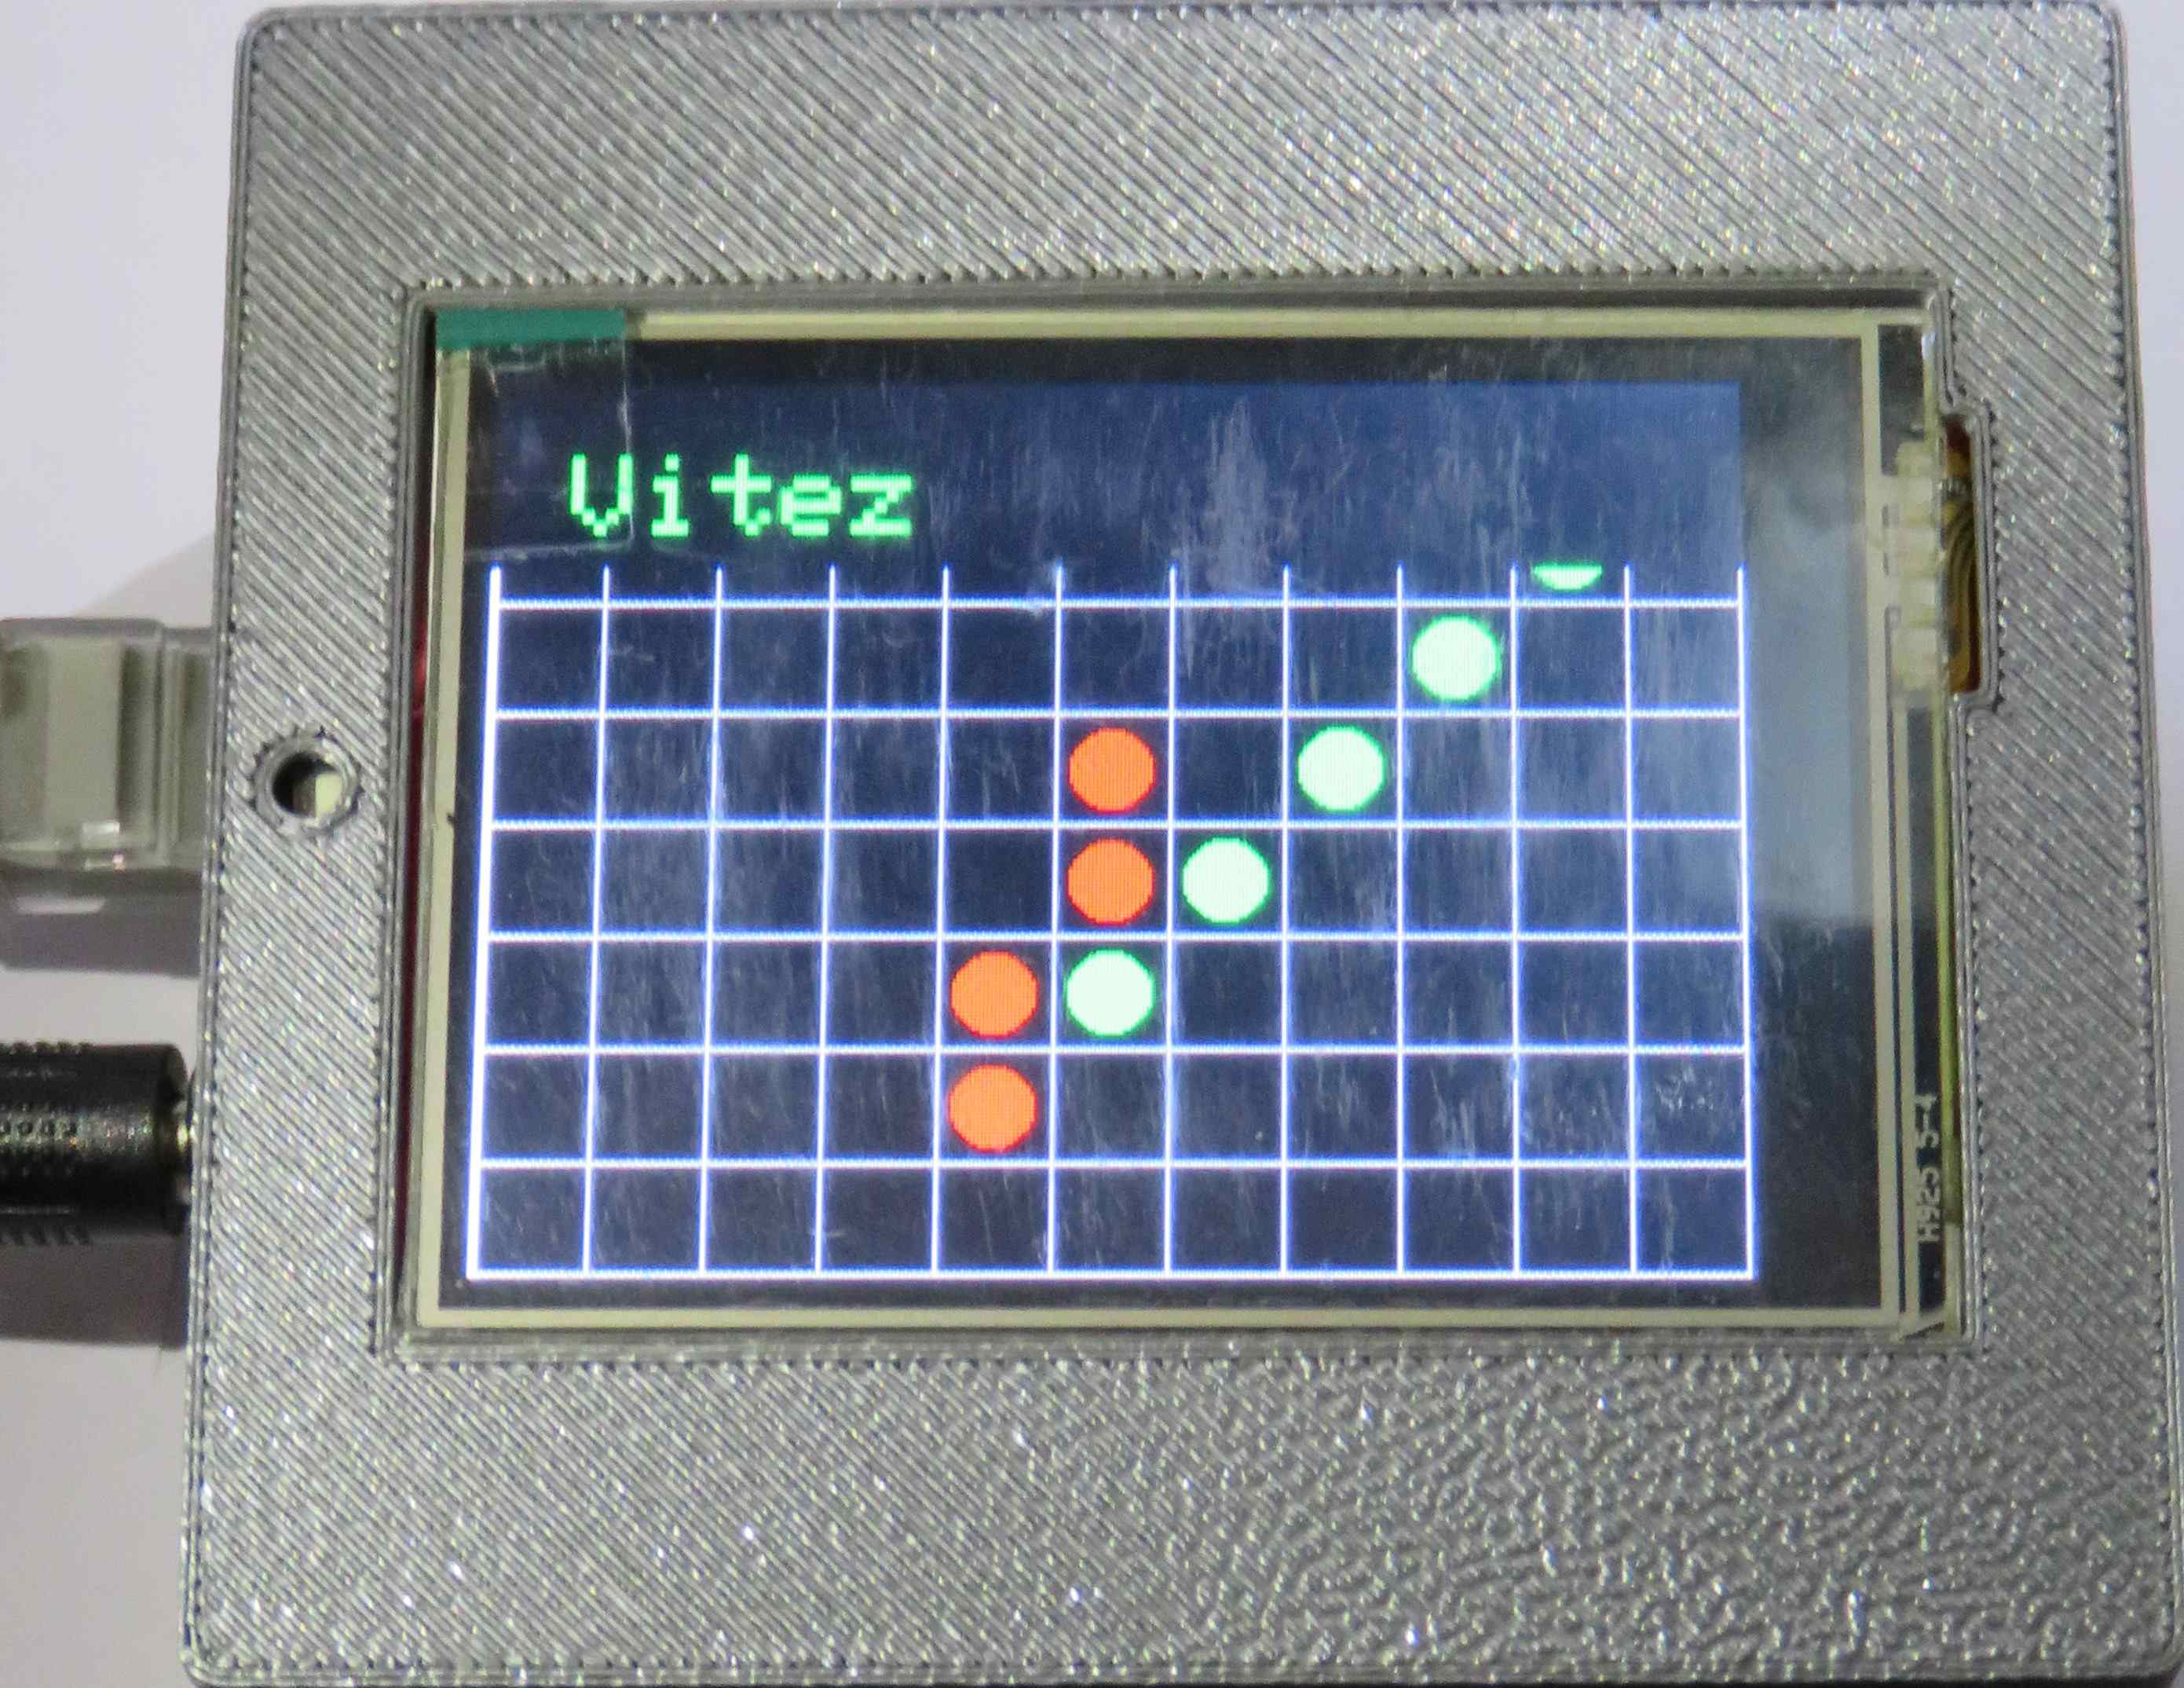
\includegraphics[width=7cm, angle=0]{img/gameFlow/phase06b.jpg}
\caption{\label{fig:faze6} Zobrazená hláška na displeji výherce (a) a ostatních hráčů (b), barva textu se shoduje s barvou vítězného hráče}
\end{figure}
\end{enumerate}
%\notFinished
\subsection{Ovládání serveru}
Server lze ovládat dvěma způsoby. Prvním z nich je ovládání pomocí dvou tlačítek.

Pokud je stisknuto červené tlačítko, dojde k přerušení hry aktuálně běžící hry (dosavadní stav hry je resetován).

Pokud je stisknuto zelené tlačítko a neběží hra (indikační LED svítí modře) - stiskem tlačítka dojde ke spuštění hry (s ověřením zda je k dispozici dostatek hráčů).
Pokud hra již běží (indikační LED svítí zeleně) stiskem zeleného tlačítka dojde k posunutí tahu na dalšího hráče.

Druhým způsobem ovládání je posílání příkazů přes sériovou linku. V tomto případě je nutné serverm připojit k počítači pomocí micro USB kabelu (konektor z přední strany serveru). K zobrazení dat lze použít nástorj \textit{Serial monitor} přímo v Arduino~IDE nebo například sériový terminál \textit{RealTerm \footnote{Domovská stránka: https://realterm.sourceforge.io/}}. Nastavení je následují: rychlost = 9600 baudů, Data bits = 8, Stop bits = 1, Flow control = none.  Každý příkaz musí být zakončen novým řádkem (LF). Seznam příkazů je v tabulce \ref{tab:server_prikazy}.

Informování uživatele o stavu serveru je realizovano pomocí barevné svítivé diody. Význa jednotlivých stavů je v tabulce \ref{tab:serverLED}. Symboly: 
\includegraphics[height=.4cm]{img/manual/blue.png} svítivá dioda svítí, 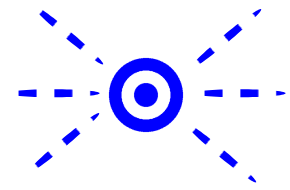
\includegraphics[height=.4cm]{img/manual/blue_blink.png} svítivá dioda bliká.

\begin{table}[hbtp]
  \centering
\caption{\label{tab:server_prikazy} Seznam příkazů dostupných pro server}
\begin{tabular}{|c|c|}
\hline
\textbf{Příkaz} & \textbf{Význam}                                        \\ \hline
help            & Vypíše nápovědu (dostupné příkazy)                     \\ \hline
info            & Vypíší informace o serveru (HW, verze SW, apod.)       \\ \hline
players         & Zobrazí čísla a IP adresy připojených hráčů            \\ \hline
kick 'x'        & Odpojí hráče číslo \textit{x}                          \\ \hline
nextP           & Přepne na dalšího hráče                                \\ \hline
start           & Spustí hru (ekvivalent zeleného tlačítka)              \\ \hline
reset           & Přeruší a resetuje hru (ekvivalent červeného tlačítka) \\ \hline
\end{tabular}
\end{table}


\begin{table}[hbtp]
\centering
\newcommand{\LEDsingHeight}{0.55cm}
\caption{Význam stavů svítivé diody na serveru, }
\label{tab:serverLED}
\label{tab:LED_man}
\begin{tabular}{|c|c|}
\hline
\textbf{Stav svítivé diody}                                            & \textbf{Význam}                  \\ \hline

\includegraphics[height=\LEDsingHeight/2]{img/manual/black.png}             & server je vypnutý/nemá napájení  \\ \hline

\includegraphics[height=\LEDsingHeight]{img/manual/blue.png}              & server je připraven              \\ \hline

\includegraphics[height=\LEDsingHeight]{img/manual/violet_blink.png} 3x   & nový klient připojen             \\ \hline

\includegraphics[height=\LEDsingHeight]{img/manual/orange_blink.png}   3x & klient se odpojil/byl odpojen    \\ \hline
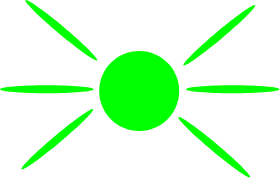
\includegraphics[height=\LEDsingHeight]{img/manual/green.png}             & aktuálně běží hra                \\ \hline

\includegraphics[height=\LEDsingHeight]{img/manual/green_blink.png}       & hra ukončena (výhra/remíza)      \\ \hline
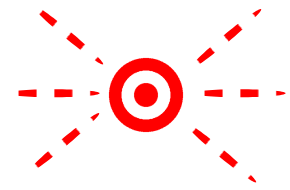
\includegraphics[height=\LEDsingHeight]{img/manual/red_blink.png} 3x      & chyba (nedostatek hráčů pro hru) \\ \hline
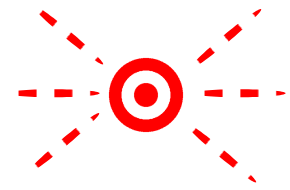
\includegraphics[height=\LEDsingHeight]{img/manual/red_blink.png} stále   & chyba sítě (připojení kabelu)    \\ \hline
\end{tabular}
\end{table}

%\notFinished
